\documentclass[a4paper]{article}
\setlength{\parskip}{11pt plus 1pt minus 1pt}

%% Language and font encodings
\usepackage[dutch]{babel}
\usepackage[utf8]{inputenc}
\usepackage[T1]{fontenc} 
\usepackage[backend=bibtex]{biblatex}
\usepackage{url}
% \addbibresource{bibliografie.bib}
\usepackage[usenames,dvipsnames]{color}


%% Sets page size and margins
\usepackage[a4paper,top=3cm,bottom=2cm,left=1in]{geometry}

%% Useful packages
\usepackage{amsmath}
\usepackage{wasysym}
\usepackage{amssymb}
\usepackage[utf8]{inputenc}
\usepackage[dutch]{babel}
\usepackage{graphicx}
\usepackage[colorinlistoftodos]{todonotes}
\usepackage[colorlinks=false, allcolors=blue]{hyperref}
\usepackage{booktabs}
\usepackage{float}
\usepackage{siunitx}
\usepackage[backend=bibtex]{biblatex}
\usepackage{subcaption}
\usepackage{gensymb}

%% tikz for plots
\usepackage{tikz}
\usetikzlibrary{external}
\tikzexternalize[prefix=plots/]
% package to determine line width
\usepackage{layouts}

\newcommand{\R}{\mathbb{R}}

\title{Take home 2}
\author{Pieter Luyten}

\begin{document}

\maketitle

\section*{Question 1}
\subsection*{(a)}
The value for the intercept of the fit is $1.0321764$ and for the rico of the fit is $0.1904323$
\begin{figure}[h]
	\centering
	% Created by tikzDevice version 0.12.3 on 2019-12-14 20:27:39
% !TEX encoding = UTF-8 Unicode
\begin{tikzpicture}[x=1pt,y=1pt]
\definecolor{fillColor}{RGB}{255,255,255}
\path[use as bounding box,fill=fillColor,fill opacity=0.00] (0,0) rectangle (392.13,304.99);
\begin{scope}
\path[clip] ( 49.20, 61.20) rectangle (366.93,255.79);
\definecolor{drawColor}{RGB}{0,0,0}
\definecolor{fillColor}{RGB}{0,0,0}

\path[draw=drawColor,line width= 0.4pt,line join=round,line cap=round,fill=fillColor] ( 60.97,160.22) circle (  1.50);

\path[draw=drawColor,line width= 0.4pt,line join=round,line cap=round,fill=fillColor] ( 67.18, 96.94) circle (  1.50);

\path[draw=drawColor,line width= 0.4pt,line join=round,line cap=round,fill=fillColor] ( 76.43,109.00) circle (  1.50);

\path[draw=drawColor,line width= 0.4pt,line join=round,line cap=round,fill=fillColor] ( 89.08,130.08) circle (  1.50);

\path[draw=drawColor,line width= 0.4pt,line join=round,line cap=round,fill=fillColor] ( 89.92,137.76) circle (  1.50);

\path[draw=drawColor,line width= 0.4pt,line join=round,line cap=round,fill=fillColor] (104.06,132.96) circle (  1.50);

\path[draw=drawColor,line width= 0.4pt,line join=round,line cap=round,fill=fillColor] (106.85,134.30) circle (  1.50);

\path[draw=drawColor,line width= 0.4pt,line join=round,line cap=round,fill=fillColor] (110.69,122.39) circle (  1.50);

\path[draw=drawColor,line width= 0.4pt,line join=round,line cap=round,fill=fillColor] (113.15,144.58) circle (  1.50);

\path[draw=drawColor,line width= 0.4pt,line join=round,line cap=round,fill=fillColor] (129.00,164.86) circle (  1.50);

\path[draw=drawColor,line width= 0.4pt,line join=round,line cap=round,fill=fillColor] (131.28,169.93) circle (  1.50);

\path[draw=drawColor,line width= 0.4pt,line join=round,line cap=round,fill=fillColor] (136.73,158.46) circle (  1.50);

\path[draw=drawColor,line width= 0.4pt,line join=round,line cap=round,fill=fillColor] (139.70,184.68) circle (  1.50);

\path[draw=drawColor,line width= 0.4pt,line join=round,line cap=round,fill=fillColor] (139.75,127.86) circle (  1.50);

\path[draw=drawColor,line width= 0.4pt,line join=round,line cap=round,fill=fillColor] (153.06, 78.70) circle (  1.50);

\path[draw=drawColor,line width= 0.4pt,line join=round,line cap=round,fill=fillColor] (155.65,183.02) circle (  1.50);

\path[draw=drawColor,line width= 0.4pt,line join=round,line cap=round,fill=fillColor] (155.77,137.33) circle (  1.50);

\path[draw=drawColor,line width= 0.4pt,line join=round,line cap=round,fill=fillColor] (167.07,127.87) circle (  1.50);

\path[draw=drawColor,line width= 0.4pt,line join=round,line cap=round,fill=fillColor] (167.72,144.54) circle (  1.50);

\path[draw=drawColor,line width= 0.4pt,line join=round,line cap=round,fill=fillColor] (168.50,195.10) circle (  1.50);

\path[draw=drawColor,line width= 0.4pt,line join=round,line cap=round,fill=fillColor] (176.11,159.76) circle (  1.50);

\path[draw=drawColor,line width= 0.4pt,line join=round,line cap=round,fill=fillColor] (181.82,155.59) circle (  1.50);

\path[draw=drawColor,line width= 0.4pt,line join=round,line cap=round,fill=fillColor] (182.73,167.54) circle (  1.50);

\path[draw=drawColor,line width= 0.4pt,line join=round,line cap=round,fill=fillColor] (193.28,136.68) circle (  1.50);

\path[draw=drawColor,line width= 0.4pt,line join=round,line cap=round,fill=fillColor] (195.23,146.54) circle (  1.50);

\path[draw=drawColor,line width= 0.4pt,line join=round,line cap=round,fill=fillColor] (203.35,139.76) circle (  1.50);

\path[draw=drawColor,line width= 0.4pt,line join=round,line cap=round,fill=fillColor] (206.39,168.82) circle (  1.50);

\path[draw=drawColor,line width= 0.4pt,line join=round,line cap=round,fill=fillColor] (212.11,146.33) circle (  1.50);

\path[draw=drawColor,line width= 0.4pt,line join=round,line cap=round,fill=fillColor] (217.63,159.23) circle (  1.50);

\path[draw=drawColor,line width= 0.4pt,line join=round,line cap=round,fill=fillColor] (227.16,144.62) circle (  1.50);

\path[draw=drawColor,line width= 0.4pt,line join=round,line cap=round,fill=fillColor] (227.62,211.65) circle (  1.50);

\path[draw=drawColor,line width= 0.4pt,line join=round,line cap=round,fill=fillColor] (230.53,164.24) circle (  1.50);

\path[draw=drawColor,line width= 0.4pt,line join=round,line cap=round,fill=fillColor] (230.71,184.31) circle (  1.50);

\path[draw=drawColor,line width= 0.4pt,line join=round,line cap=round,fill=fillColor] (238.15,135.16) circle (  1.50);

\path[draw=drawColor,line width= 0.4pt,line join=round,line cap=round,fill=fillColor] (239.00,214.61) circle (  1.50);

\path[draw=drawColor,line width= 0.4pt,line join=round,line cap=round,fill=fillColor] (257.67,154.47) circle (  1.50);

\path[draw=drawColor,line width= 0.4pt,line join=round,line cap=round,fill=fillColor] (258.95,161.21) circle (  1.50);

\path[draw=drawColor,line width= 0.4pt,line join=round,line cap=round,fill=fillColor] (263.57,142.91) circle (  1.50);

\path[draw=drawColor,line width= 0.4pt,line join=round,line cap=round,fill=fillColor] (264.26,171.19) circle (  1.50);

\path[draw=drawColor,line width= 0.4pt,line join=round,line cap=round,fill=fillColor] (265.83,172.38) circle (  1.50);

\path[draw=drawColor,line width= 0.4pt,line join=round,line cap=round,fill=fillColor] (278.68,155.57) circle (  1.50);

\path[draw=drawColor,line width= 0.4pt,line join=round,line cap=round,fill=fillColor] (279.18,156.72) circle (  1.50);

\path[draw=drawColor,line width= 0.4pt,line join=round,line cap=round,fill=fillColor] (282.81,196.42) circle (  1.50);

\path[draw=drawColor,line width= 0.4pt,line join=round,line cap=round,fill=fillColor] (282.87,137.26) circle (  1.50);

\path[draw=drawColor,line width= 0.4pt,line join=round,line cap=round,fill=fillColor] (286.59,158.47) circle (  1.50);

\path[draw=drawColor,line width= 0.4pt,line join=round,line cap=round,fill=fillColor] (289.88,172.60) circle (  1.50);

\path[draw=drawColor,line width= 0.4pt,line join=round,line cap=round,fill=fillColor] (293.32,155.89) circle (  1.50);

\path[draw=drawColor,line width= 0.4pt,line join=round,line cap=round,fill=fillColor] (300.66,159.59) circle (  1.50);

\path[draw=drawColor,line width= 0.4pt,line join=round,line cap=round,fill=fillColor] (302.12,145.32) circle (  1.50);

\path[draw=drawColor,line width= 0.4pt,line join=round,line cap=round,fill=fillColor] (302.44,134.20) circle (  1.50);

\path[draw=drawColor,line width= 0.4pt,line join=round,line cap=round,fill=fillColor] (305.09, 92.69) circle (  1.50);

\path[draw=drawColor,line width= 0.4pt,line join=round,line cap=round,fill=fillColor] (310.65,196.93) circle (  1.50);

\path[draw=drawColor,line width= 0.4pt,line join=round,line cap=round,fill=fillColor] (319.30,174.25) circle (  1.50);

\path[draw=drawColor,line width= 0.4pt,line join=round,line cap=round,fill=fillColor] (326.01,136.52) circle (  1.50);

\path[draw=drawColor,line width= 0.4pt,line join=round,line cap=round,fill=fillColor] (330.59,141.99) circle (  1.50);

\path[draw=drawColor,line width= 0.4pt,line join=round,line cap=round,fill=fillColor] (336.81,159.42) circle (  1.50);

\path[draw=drawColor,line width= 0.4pt,line join=round,line cap=round,fill=fillColor] (345.67,151.60) circle (  1.50);

\path[draw=drawColor,line width= 0.4pt,line join=round,line cap=round,fill=fillColor] (348.53,208.52) circle (  1.50);

\path[draw=drawColor,line width= 0.4pt,line join=round,line cap=round,fill=fillColor] (349.98,158.22) circle (  1.50);

\path[draw=drawColor,line width= 0.4pt,line join=round,line cap=round,fill=fillColor] (355.16,179.72) circle (  1.50);
\end{scope}
\begin{scope}
\path[clip] (  0.00,  0.00) rectangle (392.13,304.99);
\definecolor{drawColor}{RGB}{0,0,0}

\path[draw=drawColor,line width= 0.4pt,line join=round,line cap=round] ( 60.50, 61.20) -- (355.17, 61.20);

\path[draw=drawColor,line width= 0.4pt,line join=round,line cap=round] ( 60.50, 61.20) -- ( 60.50, 55.20);

\path[draw=drawColor,line width= 0.4pt,line join=round,line cap=round] (134.17, 61.20) -- (134.17, 55.20);

\path[draw=drawColor,line width= 0.4pt,line join=round,line cap=round] (207.83, 61.20) -- (207.83, 55.20);

\path[draw=drawColor,line width= 0.4pt,line join=round,line cap=round] (281.50, 61.20) -- (281.50, 55.20);

\path[draw=drawColor,line width= 0.4pt,line join=round,line cap=round] (355.17, 61.20) -- (355.17, 55.20);

\node[text=drawColor,anchor=base,inner sep=0pt, outer sep=0pt, scale=  1.00] at ( 60.50, 39.60) {-1.0};

\node[text=drawColor,anchor=base,inner sep=0pt, outer sep=0pt, scale=  1.00] at (134.17, 39.60) {-0.5};

\node[text=drawColor,anchor=base,inner sep=0pt, outer sep=0pt, scale=  1.00] at (207.83, 39.60) {0.0};

\node[text=drawColor,anchor=base,inner sep=0pt, outer sep=0pt, scale=  1.00] at (281.50, 39.60) {0.5};

\node[text=drawColor,anchor=base,inner sep=0pt, outer sep=0pt, scale=  1.00] at (355.17, 39.60) {1.0};

\path[draw=drawColor,line width= 0.4pt,line join=round,line cap=round] ( 49.20, 68.41) -- ( 49.20,232.20);

\path[draw=drawColor,line width= 0.4pt,line join=round,line cap=round] ( 49.20, 68.41) -- ( 43.20, 68.41);

\path[draw=drawColor,line width= 0.4pt,line join=round,line cap=round] ( 49.20,109.36) -- ( 43.20,109.36);

\path[draw=drawColor,line width= 0.4pt,line join=round,line cap=round] ( 49.20,150.30) -- ( 43.20,150.30);

\path[draw=drawColor,line width= 0.4pt,line join=round,line cap=round] ( 49.20,191.25) -- ( 43.20,191.25);

\path[draw=drawColor,line width= 0.4pt,line join=round,line cap=round] ( 49.20,232.20) -- ( 43.20,232.20);

\node[text=drawColor,rotate= 90.00,anchor=base,inner sep=0pt, outer sep=0pt, scale=  1.00] at ( 34.80, 68.41) {0.0};

\node[text=drawColor,rotate= 90.00,anchor=base,inner sep=0pt, outer sep=0pt, scale=  1.00] at ( 34.80,109.36) {0.5};

\node[text=drawColor,rotate= 90.00,anchor=base,inner sep=0pt, outer sep=0pt, scale=  1.00] at ( 34.80,150.30) {1.0};

\node[text=drawColor,rotate= 90.00,anchor=base,inner sep=0pt, outer sep=0pt, scale=  1.00] at ( 34.80,191.25) {1.5};

\node[text=drawColor,rotate= 90.00,anchor=base,inner sep=0pt, outer sep=0pt, scale=  1.00] at ( 34.80,232.20) {2.0};

\path[draw=drawColor,line width= 0.4pt,line join=round,line cap=round] ( 49.20, 61.20) --
	(366.93, 61.20) --
	(366.93,255.79) --
	( 49.20,255.79) --
	( 49.20, 61.20);
\end{scope}
\begin{scope}
\path[clip] (  0.00,  0.00) rectangle (392.13,304.99);
\definecolor{drawColor}{RGB}{0,0,0}

\node[text=drawColor,anchor=base,inner sep=0pt, outer sep=0pt, scale=  1.00] at (208.06, 15.60) {V1};

\node[text=drawColor,rotate= 90.00,anchor=base,inner sep=0pt, outer sep=0pt, scale=  1.00] at ( 10.80,158.49) {V2};
\end{scope}
\begin{scope}
\path[clip] ( 49.20, 61.20) rectangle (366.93,255.79);
\definecolor{drawColor}{RGB}{0,0,0}

\path[draw=drawColor,line width= 0.4pt,line join=round,line cap=round] (  0.00,130.94) --
	( 10.54,132.05) --
	( 33.78,134.51) --
	( 57.02,136.97) --
	( 80.25,139.43) --
	(103.49,141.89) --
	(126.73,144.35) --
	(149.97,146.81) --
	(173.21,149.27) --
	(196.44,151.73) --
	(219.68,154.19) --
	(242.92,156.65) --
	(266.16,159.11) --
	(289.40,161.57) --
	(312.63,164.03) --
	(335.87,166.49) --
	(359.11,168.95) --
	(382.35,171.41) --
	(392.13,172.45);
\end{scope}
\end{tikzpicture}

	\caption{line fit throught the data in Ex1.txt}
	\label{fig:fit-1a}
\end{figure}

\subsection*{(b)}
Using the result from section 7.4.1 in <REFERENCE cursus> we know that the random variable
\begin{equation}
	T = \frac{\beta_1}{\sqrt{ \frac{S^2}{ \sum_{i=1}^{n}(x_i-\bar{x}^2)}}}
\end{equation}
has a Student distribution with $n-2$ degrees of freedom. The test value is $2.603$. Using a student-t distribution with $60-2=58$ degrees of freedom we find a p-value of $0.0117$. At the confidence level $\alpha=0.01$, the null hypothesis that $\beta_1=0$ holds. The $99\%$ confidence region for the test value is $[-2.663, 2.663]$.

\subsection*{(c)}
A q-q plot is a plot where the quantiles of the assumed distribution are plotted against the quantiles from the sample. So in a sample of $n$ points where we label the observation $x_i, i \in \{1,2, \ldots, n\}$ from lowest to highest, the ith point will be plotted at the $(Q(i/n), x_i)$. 
Here $Q(x)$ is the quantile function of the assumed distribution. This is a function such that $ P( X < Q(p)) = p$. If the assumed distribution is a good model for the observed sample, the points will well fitted by a linear function.

\begin{figure}[h]
	\centering
	% Created by tikzDevice version 0.12.3 on 2019-12-10 21:17:06
% !TEX encoding = UTF-8 Unicode
\begin{tikzpicture}[x=1pt,y=1pt]
\definecolor{fillColor}{RGB}{255,255,255}
\path[use as bounding box,fill=fillColor,fill opacity=0.00] (0,0) rectangle (392.13,304.99);
\begin{scope}
\path[clip] ( 49.20, 61.20) rectangle (366.93,255.79);
\definecolor{drawColor}{RGB}{0,0,0}

\path[draw=drawColor,line width= 0.4pt,line join=round,line cap=round] (265.49,198.91) circle (  2.25);

\path[draw=drawColor,line width= 0.4pt,line join=round,line cap=round] (101.66,109.54) circle (  2.25);

\path[draw=drawColor,line width= 0.4pt,line join=round,line cap=round] (111.66,125.02) circle (  2.25);

\path[draw=drawColor,line width= 0.4pt,line join=round,line cap=round] (177.31,152.62) circle (  2.25);

\path[draw=drawColor,line width= 0.4pt,line join=round,line cap=round] (217.08,163.23) circle (  2.25);

\path[draw=drawColor,line width= 0.4pt,line join=round,line cap=round] (185.76,154.42) circle (  2.25);

\path[draw=drawColor,line width= 0.4pt,line join=round,line cap=round] (188.48,155.88) circle (  2.25);

\path[draw=drawColor,line width= 0.4pt,line join=round,line cap=round] (150.64,138.68) circle (  2.25);

\path[draw=drawColor,line width= 0.4pt,line join=round,line cap=round] (219.68,169.33) circle (  2.25);

\path[draw=drawColor,line width= 0.4pt,line join=round,line cap=round] (261.63,195.32) circle (  2.25);

\path[draw=drawColor,line width= 0.4pt,line join=round,line cap=round] (269.59,202.07) circle (  2.25);

\path[draw=drawColor,line width= 0.4pt,line join=round,line cap=round] (247.91,185.23) circle (  2.25);

\path[draw=drawColor,line width= 0.4pt,line join=round,line cap=round] (296.51,221.44) circle (  2.25);

\path[draw=drawColor,line width= 0.4pt,line join=round,line cap=round] (154.50,142.02) circle (  2.25);

\path[draw=drawColor,line width= 0.4pt,line join=round,line cap=round] ( 87.64, 71.34) circle (  2.25);

\path[draw=drawColor,line width= 0.4pt,line join=round,line cap=round] (289.82,216.76) circle (  2.25);

\path[draw=drawColor,line width= 0.4pt,line join=round,line cap=round] (180.18,152.88) circle (  2.25);

\path[draw=drawColor,line width= 0.4pt,line join=round,line cap=round] (146.54,137.99) circle (  2.25);

\path[draw=drawColor,line width= 0.4pt,line join=round,line cap=round] (204.21,161.19) circle (  2.25);

\path[draw=drawColor,line width= 0.4pt,line join=round,line cap=round] (314.46,231.74) circle (  2.25);

\path[draw=drawColor,line width= 0.4pt,line join=round,line cap=round] (235.94,181.23) circle (  2.25);

\path[draw=drawColor,line width= 0.4pt,line join=round,line cap=round] (227.64,174.56) circle (  2.25);

\path[draw=drawColor,line width= 0.4pt,line join=round,line cap=round] (257.97,191.12) circle (  2.25);

\path[draw=drawColor,line width= 0.4pt,line join=round,line cap=round] (168.22,146.43) circle (  2.25);

\path[draw=drawColor,line width= 0.4pt,line join=round,line cap=round] (199.05,159.93) circle (  2.25);

\path[draw=drawColor,line width= 0.4pt,line join=round,line cap=round] (171.33,149.25) circle (  2.25);

\path[draw=drawColor,line width= 0.4pt,line join=round,line cap=round] (254.48,189.41) circle (  2.25);

\path[draw=drawColor,line width= 0.4pt,line join=round,line cap=round] (193.82,157.12) circle (  2.25);

\path[draw=drawColor,line width= 0.4pt,line join=round,line cap=round] (224.96,174.34) circle (  2.25);

\path[draw=drawColor,line width= 0.4pt,line join=round,line cap=round] (174.36,152.51) circle (  2.25);

\path[draw=drawColor,line width= 0.4pt,line join=round,line cap=round] (328.49,246.13) circle (  2.25);

\path[draw=drawColor,line width= 0.4pt,line join=round,line cap=round] (230.36,179.43) circle (  2.25);

\path[draw=drawColor,line width= 0.4pt,line join=round,line cap=round] (273.98,207.46) circle (  2.25);

\path[draw=drawColor,line width= 0.4pt,line join=round,line cap=round] (142.14,137.66) circle (  2.25);

\path[draw=drawColor,line width= 0.4pt,line join=round,line cap=round] (355.16,248.58) circle (  2.25);

\path[draw=drawColor,line width= 0.4pt,line join=round,line cap=round] (209.35,161.77) circle (  2.25);

\path[draw=drawColor,line width= 0.4pt,line join=round,line cap=round] (222.31,171.00) circle (  2.25);

\path[draw=drawColor,line width= 0.4pt,line join=round,line cap=round] (164.99,144.74) circle (  2.25);

\path[draw=drawColor,line width= 0.4pt,line join=round,line cap=round] (244.79,184.16) circle (  2.25);

\path[draw=drawColor,line width= 0.4pt,line join=round,line cap=round] (251.13,185.59) circle (  2.25);

\path[draw=drawColor,line width= 0.4pt,line join=round,line cap=round] (201.63,160.19) circle (  2.25);

\path[draw=drawColor,line width= 0.4pt,line join=round,line cap=round] (206.78,161.73) circle (  2.25);

\path[draw=drawColor,line width= 0.4pt,line join=round,line cap=round] (283.97,216.68) circle (  2.25);

\path[draw=drawColor,line width= 0.4pt,line join=round,line cap=round] (137.38,133.99) circle (  2.25);

\path[draw=drawColor,line width= 0.4pt,line join=round,line cap=round] (214.49,163.07) circle (  2.25);

\path[draw=drawColor,line width= 0.4pt,line join=round,line cap=round] (238.82,182.34) circle (  2.25);

\path[draw=drawColor,line width= 0.4pt,line join=round,line cap=round] (196.44,158.47) circle (  2.25);

\path[draw=drawColor,line width= 0.4pt,line join=round,line cap=round] (211.92,162.56) circle (  2.25);

\path[draw=drawColor,line width= 0.4pt,line join=round,line cap=round] (158.16,142.40) circle (  2.25);

\path[draw=drawColor,line width= 0.4pt,line join=round,line cap=round] (126.31,126.81) circle (  2.25);

\path[draw=drawColor,line width= 0.4pt,line join=round,line cap=round] ( 60.97, 68.41) circle (  2.25);

\path[draw=drawColor,line width= 0.4pt,line join=round,line cap=round] (278.74,213.27) circle (  2.25);

\path[draw=drawColor,line width= 0.4pt,line join=round,line cap=round] (233.13,180.30) circle (  2.25);

\path[draw=drawColor,line width= 0.4pt,line join=round,line cap=round] (119.61,126.57) circle (  2.25);

\path[draw=drawColor,line width= 0.4pt,line join=round,line cap=round] (132.15,133.53) circle (  2.25);

\path[draw=drawColor,line width= 0.4pt,line join=round,line cap=round] (191.17,156.97) circle (  2.25);

\path[draw=drawColor,line width= 0.4pt,line join=round,line cap=round] (161.65,144.73) circle (  2.25);

\path[draw=drawColor,line width= 0.4pt,line join=round,line cap=round] (304.46,223.86) circle (  2.25);

\path[draw=drawColor,line width= 0.4pt,line join=round,line cap=round] (183.00,153.35) circle (  2.25);

\path[draw=drawColor,line width= 0.4pt,line join=round,line cap=round] (241.77,182.64) circle (  2.25);
\end{scope}
\begin{scope}
\path[clip] (  0.00,  0.00) rectangle (392.13,304.99);
\definecolor{drawColor}{RGB}{0,0,0}

\path[draw=drawColor,line width= 0.4pt,line join=round,line cap=round] ( 85.18, 61.20) -- (330.95, 61.20);

\path[draw=drawColor,line width= 0.4pt,line join=round,line cap=round] ( 85.18, 61.20) -- ( 85.18, 55.20);

\path[draw=drawColor,line width= 0.4pt,line join=round,line cap=round] (146.62, 61.20) -- (146.62, 55.20);

\path[draw=drawColor,line width= 0.4pt,line join=round,line cap=round] (208.06, 61.20) -- (208.06, 55.20);

\path[draw=drawColor,line width= 0.4pt,line join=round,line cap=round] (269.51, 61.20) -- (269.51, 55.20);

\path[draw=drawColor,line width= 0.4pt,line join=round,line cap=round] (330.95, 61.20) -- (330.95, 55.20);

\node[text=drawColor,anchor=base,inner sep=0pt, outer sep=0pt, scale=  1.00] at ( 85.18, 39.60) {-2};

\node[text=drawColor,anchor=base,inner sep=0pt, outer sep=0pt, scale=  1.00] at (146.62, 39.60) {-1};

\node[text=drawColor,anchor=base,inner sep=0pt, outer sep=0pt, scale=  1.00] at (208.06, 39.60) {0};

\node[text=drawColor,anchor=base,inner sep=0pt, outer sep=0pt, scale=  1.00] at (269.51, 39.60) {1};

\node[text=drawColor,anchor=base,inner sep=0pt, outer sep=0pt, scale=  1.00] at (330.95, 39.60) {2};

\path[draw=drawColor,line width= 0.4pt,line join=round,line cap=round] ( 49.20,109.77) -- ( 49.20,224.23);

\path[draw=drawColor,line width= 0.4pt,line join=round,line cap=round] ( 49.20,109.77) -- ( 43.20,109.77);

\path[draw=drawColor,line width= 0.4pt,line join=round,line cap=round] ( 49.20,167.00) -- ( 43.20,167.00);

\path[draw=drawColor,line width= 0.4pt,line join=round,line cap=round] ( 49.20,224.23) -- ( 43.20,224.23);

\node[text=drawColor,rotate= 90.00,anchor=base,inner sep=0pt, outer sep=0pt, scale=  1.00] at ( 34.80,109.77) {-0.5};

\node[text=drawColor,rotate= 90.00,anchor=base,inner sep=0pt, outer sep=0pt, scale=  1.00] at ( 34.80,167.00) {0.0};

\node[text=drawColor,rotate= 90.00,anchor=base,inner sep=0pt, outer sep=0pt, scale=  1.00] at ( 34.80,224.23) {0.5};

\path[draw=drawColor,line width= 0.4pt,line join=round,line cap=round] ( 49.20, 61.20) --
	(366.93, 61.20) --
	(366.93,255.79) --
	( 49.20,255.79) --
	( 49.20, 61.20);
\end{scope}
\begin{scope}
\path[clip] (  0.00,  0.00) rectangle (392.13,304.99);
\definecolor{drawColor}{RGB}{0,0,0}

\node[text=drawColor,anchor=base,inner sep=0pt, outer sep=0pt, scale=  1.20] at (208.06,276.25) {\bfseries Normal Q-Q Plot};

\node[text=drawColor,anchor=base,inner sep=0pt, outer sep=0pt, scale=  1.00] at (208.06, 15.60) {Theoretical Quantiles};

\node[text=drawColor,rotate= 90.00,anchor=base,inner sep=0pt, outer sep=0pt, scale=  1.00] at ( 10.80,158.49) {Sample Quantiles};
\end{scope}
\begin{scope}
\path[clip] ( 49.20, 61.20) rectangle (366.93,255.79);
\definecolor{drawColor}{RGB}{0,0,0}

\path[draw=drawColor,line width= 0.4pt,line join=round,line cap=round] ( 49.20, 90.31) -- (366.93,241.01);
\end{scope}
\end{tikzpicture}

	\caption{qq plot for the errors on the fit}
	\label{fig:qqplot-1c}
\end{figure}

\subsection*{(d)}
We use the formula from section 7.5.4 in the book to find a confidence region for $\mathbf{\beta}$. THis region is of the form:
\begin{equation}
	\left\{ \beta \bigg| \frac{(\hat{\beta}-\beta)^T (X^TX) (\hat{\beta}-\beta)}{pS^2} \leq F_{p,n-p}(1-\alpha) \right\}
\end{equation}
Because the matrix $X^TX$ is positive definite, this is an ellips with center $\mathbf{\beta}$ and axes along the eigenvectors of $X^TX$. The upper bound for this expression is in this case: $F_{2,58(0.99) = 4.9910}$ Filling in the values for $X, p=2, n=60$ and $S^2$ we get the following result (obtained using the cAS system sympy):
\begin{equation*}
	\{ \beta | 5.2596 \alpha^{2} + 0.8222 \alpha \beta - 0.4950 \alpha + 1.6711 \beta^{2} - 0.6629 \beta + 0.0711 \leq 4.9910 \}
\end{equation*}


\section*{Question 2}

\subsection*{(a)}
The value for $\hat{\beta}_{OLS}$ obtained using ordinary least squares with the correlated errors is:
\begin{equation}
	\hat{\beta}_{OLS} = (3.923161, 1.214355)^T
\end{equation}

\subsection*{(b)}
we know that the variance is the same for all $\epsilon_i$ and that they obey the recursive relation:
\begin{equation*}
	\epsilon_i = \rho \epsilon_{i-1} + \eta_i
\end{equation*}
with $\eta_i$ standard normaly distributed. Using $Var(\epsilon_i) =Var(\epsilon_j)$ for all $i, j \in \{1, 2, \ldots 80\}$ we find:
\begin{align*}
	Var(\epsilon_i) &= \rho^2 Var(\epsilon_{i-1}) + Var(\eta_i)\\
	\Leftrightarrow Var(\epsilon_i) &= \rho^2 Var(\epsilon_i) + 1\\
	\Leftrightarrow Var(\epsilon_i) &= \frac{1}{1-\rho^2}\\
					&= \frac{25}{9}\\
					&= 2.777 \ldots
\end{align*}
We conclude that the variance of $\epsilon$ is $ \frac{25}{9}$.

\subsection*{(c)}
To transform the errors to a basis where they are no longer correlated we will use the variance-covariance matrix $V$ of the errors. 
The off-diagonal elements, so the covariances, are (suppose $i < j$:
\begin{align*}
	Cov(\epsilon_i, \epsilon_j) &= E[(\epsilon_i-E(\epsilon_i))(\epsilon_j-E(epsilon_j))]\\
				    &= E[\epsilon_i \epsilon_j]\\
				    &= E[\epsilon_i (\rho\epsilon_{j-1} \eta_j)]\\
				    &\vdots\\
				    &= E[\epsilon_i (\rho^{j-i} \epsilon_i + \rho^{j-i-1}\eta_i + \rho^{j-i-2}\eta_{i-2} + \ldots + \eta_j)]\\
				    &= E[\epsilon_i \rho^{i-j} \epsilon_i]\\
				    &= \rho^{i-j} Var(\epsilon)\\
				    &= \rho^{i-j} \frac{25}{9}
\end{align*}
So the matrix V has $ \frac{25}{9}$ on the diagonal, $ \frac{25}{9}\rho $ on the two sub-diagonals next to the diagonal, $ \frac{25}{9} \rho^k$ on the $k$th sub-diagonal.
the matrix $V$ can be diagonalized with an orthogonal (or unitary) transformation $U$: $\Lambda = MVM^T$. When we use the definition of the variance-covariance matrix (where $\mathbf{\epsilon}$ denotes the column vector with the errors) we find:
\begin{align*}
	V &= E( (\mathbf{\epsilon} - E(\mathbf{\epsilon})) (\mathbf{\epsilon} - E(\mathbf{\epsilon}))^T)\\
	\Leftrightarrow \Lambda &= U E( \mathbf{\epsilon} \mathbf{\epsilon}^T) U^T\\
	\Leftrightarrow \Lambda &= E( (U\mathbf{\epsilon})(U\mathbf{\epsilon})^T)\\
\end{align*}
Where we used that $E(\mathbf{\epsilon} = \mathbf{0})$. The vector $U \mathbf{\epsilon}$ has variance-covariance matrix $\Lambda$ so we conclude that it is a vector of uncorrelated stochastic variables.

The value for $\hat{\beta}_{OLS}$ that we find using these uncorrelated errors is exactly the same as with the uncorrelated errors:
\begin{equation*}
	\hat{\beta}_{OLS} = (3.923161, 1.214355)^T
\end{equation*}
This is expected because we used a unitary transformation to get uncorrelated errors and by filling this in the expression for the Sum of squares of the remainders we find:
\begin{align*}
	RSS(\hat{\beta}_{Uncorrelated}) &= (UY-UX\beta)^T(UY-UX\beta)\\
		   &= (Y-X\beta)^T U^T U (Y-X\beta)\\
		   &= (Y-X\beta)^T I (Y-X\beta)\\
		   &= RSS(\hat{\beta}_{Correlated})
\end{align*}
which means the RSS for the correlated and the uncorrelated errors will have the same optimal $\hat{\beta}$.

\section*{Question 3}

\subsection*{(a)}
The values for the fitted coefficients with ordinary least squares are: $[0.4994, 1.1985, -2.4959, 1.2082]$. In figure \ref{fig:fit-3} the fit is plotted along with the data. 
\begin{figure}
	\centering
	% Created by tikzDevice version 0.12.3 on 2019-12-11 20:36:26
% !TEX encoding = UTF-8 Unicode
\begin{tikzpicture}[x=1pt,y=1pt]
\definecolor{fillColor}{RGB}{255,255,255}
\path[use as bounding box,fill=fillColor,fill opacity=0.00] (0,0) rectangle (392.13,304.99);
\begin{scope}
\path[clip] ( 49.20, 61.20) rectangle (366.93,255.79);
\definecolor{drawColor}{RGB}{0,255,0}
\definecolor{fillColor}{RGB}{0,255,0}

\path[draw=drawColor,line width= 0.4pt,line join=round,line cap=round,fill=fillColor] ( 60.97,168.42) circle (  1.50);

\path[draw=drawColor,line width= 0.4pt,line join=round,line cap=round,fill=fillColor] ( 63.44,169.00) circle (  1.50);

\path[draw=drawColor,line width= 0.4pt,line join=round,line cap=round,fill=fillColor] ( 65.91,169.36) circle (  1.50);

\path[draw=drawColor,line width= 0.4pt,line join=round,line cap=round,fill=fillColor] ( 68.38,169.83) circle (  1.50);

\path[draw=drawColor,line width= 0.4pt,line join=round,line cap=round,fill=fillColor] ( 70.86,170.57) circle (  1.50);

\path[draw=drawColor,line width= 0.4pt,line join=round,line cap=round,fill=fillColor] ( 73.33,171.04) circle (  1.50);

\path[draw=drawColor,line width= 0.4pt,line join=round,line cap=round,fill=fillColor] ( 75.80,171.11) circle (  1.50);

\path[draw=drawColor,line width= 0.4pt,line join=round,line cap=round,fill=fillColor] ( 78.27,171.51) circle (  1.50);

\path[draw=drawColor,line width= 0.4pt,line join=round,line cap=round,fill=fillColor] ( 80.75,170.98) circle (  1.50);

\path[draw=drawColor,line width= 0.4pt,line join=round,line cap=round,fill=fillColor] ( 83.22,171.11) circle (  1.50);

\path[draw=drawColor,line width= 0.4pt,line join=round,line cap=round,fill=fillColor] ( 85.69,170.84) circle (  1.50);

\path[draw=drawColor,line width= 0.4pt,line join=round,line cap=round,fill=fillColor] ( 88.16,169.89) circle (  1.50);

\path[draw=drawColor,line width= 0.4pt,line join=round,line cap=round,fill=fillColor] ( 90.63,173.21) circle (  1.50);

\path[draw=drawColor,line width= 0.4pt,line join=round,line cap=round,fill=fillColor] ( 93.11,174.38) circle (  1.50);

\path[draw=drawColor,line width= 0.4pt,line join=round,line cap=round,fill=fillColor] ( 95.58,174.45) circle (  1.50);

\path[draw=drawColor,line width= 0.4pt,line join=round,line cap=round,fill=fillColor] ( 98.05,171.87) circle (  1.50);

\path[draw=drawColor,line width= 0.4pt,line join=round,line cap=round,fill=fillColor] (100.52,170.74) circle (  1.50);

\path[draw=drawColor,line width= 0.4pt,line join=round,line cap=round,fill=fillColor] (102.99,172.39) circle (  1.50);

\path[draw=drawColor,line width= 0.4pt,line join=round,line cap=round,fill=fillColor] (105.47,180.23) circle (  1.50);

\path[draw=drawColor,line width= 0.4pt,line join=round,line cap=round,fill=fillColor] (107.94,168.91) circle (  1.50);

\path[draw=drawColor,line width= 0.4pt,line join=round,line cap=round,fill=fillColor] (110.41,173.95) circle (  1.50);

\path[draw=drawColor,line width= 0.4pt,line join=round,line cap=round,fill=fillColor] (112.88,183.76) circle (  1.50);

\path[draw=drawColor,line width= 0.4pt,line join=round,line cap=round,fill=fillColor] (115.36,169.56) circle (  1.50);

\path[draw=drawColor,line width= 0.4pt,line join=round,line cap=round,fill=fillColor] (117.83,177.93) circle (  1.50);

\path[draw=drawColor,line width= 0.4pt,line join=round,line cap=round,fill=fillColor] (120.30,174.85) circle (  1.50);

\path[draw=drawColor,line width= 0.4pt,line join=round,line cap=round,fill=fillColor] (122.77,173.32) circle (  1.50);

\path[draw=drawColor,line width= 0.4pt,line join=round,line cap=round,fill=fillColor] (125.24,163.92) circle (  1.50);

\path[draw=drawColor,line width= 0.4pt,line join=round,line cap=round,fill=fillColor] (127.72,176.44) circle (  1.50);

\path[draw=drawColor,line width= 0.4pt,line join=round,line cap=round,fill=fillColor] (130.19,160.03) circle (  1.50);

\path[draw=drawColor,line width= 0.4pt,line join=round,line cap=round,fill=fillColor] (132.66,185.25) circle (  1.50);

\path[draw=drawColor,line width= 0.4pt,line join=round,line cap=round,fill=fillColor] (135.13,174.50) circle (  1.50);

\path[draw=drawColor,line width= 0.4pt,line join=round,line cap=round,fill=fillColor] (137.61,194.59) circle (  1.50);

\path[draw=drawColor,line width= 0.4pt,line join=round,line cap=round,fill=fillColor] (140.08,169.23) circle (  1.50);

\path[draw=drawColor,line width= 0.4pt,line join=round,line cap=round,fill=fillColor] (142.55,167.61) circle (  1.50);

\path[draw=drawColor,line width= 0.4pt,line join=round,line cap=round,fill=fillColor] (145.02,180.61) circle (  1.50);

\path[draw=drawColor,line width= 0.4pt,line join=round,line cap=round,fill=fillColor] (147.49,170.89) circle (  1.50);

\path[draw=drawColor,line width= 0.4pt,line join=round,line cap=round,fill=fillColor] (149.97,164.41) circle (  1.50);

\path[draw=drawColor,line width= 0.4pt,line join=round,line cap=round,fill=fillColor] (152.44,178.31) circle (  1.50);

\path[draw=drawColor,line width= 0.4pt,line join=round,line cap=round,fill=fillColor] (154.91,190.57) circle (  1.50);

\path[draw=drawColor,line width= 0.4pt,line join=round,line cap=round,fill=fillColor] (157.38,167.10) circle (  1.50);

\path[draw=drawColor,line width= 0.4pt,line join=round,line cap=round,fill=fillColor] (159.86,170.14) circle (  1.50);

\path[draw=drawColor,line width= 0.4pt,line join=round,line cap=round,fill=fillColor] (162.33,188.47) circle (  1.50);

\path[draw=drawColor,line width= 0.4pt,line join=round,line cap=round,fill=fillColor] (164.80,155.18) circle (  1.50);

\path[draw=drawColor,line width= 0.4pt,line join=round,line cap=round,fill=fillColor] (167.27,197.79) circle (  1.50);

\path[draw=drawColor,line width= 0.4pt,line join=round,line cap=round,fill=fillColor] (169.74,186.79) circle (  1.50);

\path[draw=drawColor,line width= 0.4pt,line join=round,line cap=round,fill=fillColor] (172.22,164.72) circle (  1.50);

\path[draw=drawColor,line width= 0.4pt,line join=round,line cap=round,fill=fillColor] (174.69,106.11) circle (  1.50);

\path[draw=drawColor,line width= 0.4pt,line join=round,line cap=round,fill=fillColor] (177.16,168.06) circle (  1.50);

\path[draw=drawColor,line width= 0.4pt,line join=round,line cap=round,fill=fillColor] (179.63,152.30) circle (  1.50);

\path[draw=drawColor,line width= 0.4pt,line join=round,line cap=round,fill=fillColor] (182.11,160.71) circle (  1.50);

\path[draw=drawColor,line width= 0.4pt,line join=round,line cap=round,fill=fillColor] (184.58,164.54) circle (  1.50);

\path[draw=drawColor,line width= 0.4pt,line join=round,line cap=round,fill=fillColor] (187.05,154.65) circle (  1.50);

\path[draw=drawColor,line width= 0.4pt,line join=round,line cap=round,fill=fillColor] (189.52,185.03) circle (  1.50);

\path[draw=drawColor,line width= 0.4pt,line join=round,line cap=round,fill=fillColor] (191.99,190.32) circle (  1.50);

\path[draw=drawColor,line width= 0.4pt,line join=round,line cap=round,fill=fillColor] (194.47,203.25) circle (  1.50);

\path[draw=drawColor,line width= 0.4pt,line join=round,line cap=round,fill=fillColor] (196.94,196.82) circle (  1.50);

\path[draw=drawColor,line width= 0.4pt,line join=round,line cap=round,fill=fillColor] (199.41,160.09) circle (  1.50);

\path[draw=drawColor,line width= 0.4pt,line join=round,line cap=round,fill=fillColor] (201.88, 95.93) circle (  1.50);

\path[draw=drawColor,line width= 0.4pt,line join=round,line cap=round,fill=fillColor] (204.35,144.77) circle (  1.50);

\path[draw=drawColor,line width= 0.4pt,line join=round,line cap=round,fill=fillColor] (206.83,140.72) circle (  1.50);

\path[draw=drawColor,line width= 0.4pt,line join=round,line cap=round,fill=fillColor] (209.30,164.42) circle (  1.50);

\path[draw=drawColor,line width= 0.4pt,line join=round,line cap=round,fill=fillColor] (211.77,141.39) circle (  1.50);

\path[draw=drawColor,line width= 0.4pt,line join=round,line cap=round,fill=fillColor] (214.24,228.38) circle (  1.50);

\path[draw=drawColor,line width= 0.4pt,line join=round,line cap=round,fill=fillColor] (216.72,134.95) circle (  1.50);

\path[draw=drawColor,line width= 0.4pt,line join=round,line cap=round,fill=fillColor] (219.19,161.14) circle (  1.50);

\path[draw=drawColor,line width= 0.4pt,line join=round,line cap=round,fill=fillColor] (221.66,118.35) circle (  1.50);

\path[draw=drawColor,line width= 0.4pt,line join=round,line cap=round,fill=fillColor] (224.13,234.40) circle (  1.50);

\path[draw=drawColor,line width= 0.4pt,line join=round,line cap=round,fill=fillColor] (226.60,245.10) circle (  1.50);

\path[draw=drawColor,line width= 0.4pt,line join=round,line cap=round,fill=fillColor] (229.08,164.23) circle (  1.50);

\path[draw=drawColor,line width= 0.4pt,line join=round,line cap=round,fill=fillColor] (231.55,146.08) circle (  1.50);

\path[draw=drawColor,line width= 0.4pt,line join=round,line cap=round,fill=fillColor] (234.02,105.78) circle (  1.50);

\path[draw=drawColor,line width= 0.4pt,line join=round,line cap=round,fill=fillColor] (236.49,177.28) circle (  1.50);

\path[draw=drawColor,line width= 0.4pt,line join=round,line cap=round,fill=fillColor] (238.97, 68.41) circle (  1.50);

\path[draw=drawColor,line width= 0.4pt,line join=round,line cap=round,fill=fillColor] (241.44,109.00) circle (  1.50);

\path[draw=drawColor,line width= 0.4pt,line join=round,line cap=round,fill=fillColor] (243.91,221.04) circle (  1.50);

\path[draw=drawColor,line width= 0.4pt,line join=round,line cap=round,fill=fillColor] (246.38,159.66) circle (  1.50);

\path[draw=drawColor,line width= 0.4pt,line join=round,line cap=round,fill=fillColor] (248.85,151.47) circle (  1.50);

\path[draw=drawColor,line width= 0.4pt,line join=round,line cap=round,fill=fillColor] (251.33,166.43) circle (  1.50);

\path[draw=drawColor,line width= 0.4pt,line join=round,line cap=round,fill=fillColor] (253.80,146.73) circle (  1.50);

\path[draw=drawColor,line width= 0.4pt,line join=round,line cap=round,fill=fillColor] (256.27,205.56) circle (  1.50);

\path[draw=drawColor,line width= 0.4pt,line join=round,line cap=round,fill=fillColor] (258.74,171.77) circle (  1.50);

\path[draw=drawColor,line width= 0.4pt,line join=round,line cap=round,fill=fillColor] (261.22,213.76) circle (  1.50);

\path[draw=drawColor,line width= 0.4pt,line join=round,line cap=round,fill=fillColor] (263.69,179.22) circle (  1.50);

\path[draw=drawColor,line width= 0.4pt,line join=round,line cap=round,fill=fillColor] (266.16,130.02) circle (  1.50);

\path[draw=drawColor,line width= 0.4pt,line join=round,line cap=round,fill=fillColor] (268.63,147.63) circle (  1.50);

\path[draw=drawColor,line width= 0.4pt,line join=round,line cap=round,fill=fillColor] (271.10,222.61) circle (  1.50);

\path[draw=drawColor,line width= 0.4pt,line join=round,line cap=round,fill=fillColor] (273.58,248.58) circle (  1.50);

\path[draw=drawColor,line width= 0.4pt,line join=round,line cap=round,fill=fillColor] (276.05,164.94) circle (  1.50);

\path[draw=drawColor,line width= 0.4pt,line join=round,line cap=round,fill=fillColor] (278.52,151.85) circle (  1.50);

\path[draw=drawColor,line width= 0.4pt,line join=round,line cap=round,fill=fillColor] (280.99,243.46) circle (  1.50);

\path[draw=drawColor,line width= 0.4pt,line join=round,line cap=round,fill=fillColor] (283.46,127.97) circle (  1.50);

\path[draw=drawColor,line width= 0.4pt,line join=round,line cap=round,fill=fillColor] (285.94,184.54) circle (  1.50);

\path[draw=drawColor,line width= 0.4pt,line join=round,line cap=round,fill=fillColor] (288.41,185.97) circle (  1.50);

\path[draw=drawColor,line width= 0.4pt,line join=round,line cap=round,fill=fillColor] (290.88,190.33) circle (  1.50);

\path[draw=drawColor,line width= 0.4pt,line join=round,line cap=round,fill=fillColor] (293.35,172.41) circle (  1.50);

\path[draw=drawColor,line width= 0.4pt,line join=round,line cap=round,fill=fillColor] (295.83,201.31) circle (  1.50);

\path[draw=drawColor,line width= 0.4pt,line join=round,line cap=round,fill=fillColor] (298.30,189.48) circle (  1.50);

\path[draw=drawColor,line width= 0.4pt,line join=round,line cap=round,fill=fillColor] (300.77,178.48) circle (  1.50);

\path[draw=drawColor,line width= 0.4pt,line join=round,line cap=round,fill=fillColor] (303.24,164.24) circle (  1.50);

\path[draw=drawColor,line width= 0.4pt,line join=round,line cap=round,fill=fillColor] (305.71,193.33) circle (  1.50);

\path[draw=drawColor,line width= 0.4pt,line join=round,line cap=round,fill=fillColor] (308.19,196.00) circle (  1.50);

\path[draw=drawColor,line width= 0.4pt,line join=round,line cap=round,fill=fillColor] (310.66,199.24) circle (  1.50);

\path[draw=drawColor,line width= 0.4pt,line join=round,line cap=round,fill=fillColor] (313.13,186.53) circle (  1.50);

\path[draw=drawColor,line width= 0.4pt,line join=round,line cap=round,fill=fillColor] (315.60,182.58) circle (  1.50);

\path[draw=drawColor,line width= 0.4pt,line join=round,line cap=round,fill=fillColor] (318.08,202.74) circle (  1.50);

\path[draw=drawColor,line width= 0.4pt,line join=round,line cap=round,fill=fillColor] (320.55,216.00) circle (  1.50);

\path[draw=drawColor,line width= 0.4pt,line join=round,line cap=round,fill=fillColor] (323.02,204.43) circle (  1.50);

\path[draw=drawColor,line width= 0.4pt,line join=round,line cap=round,fill=fillColor] (325.49,208.80) circle (  1.50);

\path[draw=drawColor,line width= 0.4pt,line join=round,line cap=round,fill=fillColor] (327.96,207.23) circle (  1.50);

\path[draw=drawColor,line width= 0.4pt,line join=round,line cap=round,fill=fillColor] (330.44,212.38) circle (  1.50);

\path[draw=drawColor,line width= 0.4pt,line join=round,line cap=round,fill=fillColor] (332.91,221.30) circle (  1.50);

\path[draw=drawColor,line width= 0.4pt,line join=round,line cap=round,fill=fillColor] (335.38,219.07) circle (  1.50);

\path[draw=drawColor,line width= 0.4pt,line join=round,line cap=round,fill=fillColor] (337.85,215.87) circle (  1.50);

\path[draw=drawColor,line width= 0.4pt,line join=round,line cap=round,fill=fillColor] (340.33,221.50) circle (  1.50);

\path[draw=drawColor,line width= 0.4pt,line join=round,line cap=round,fill=fillColor] (342.80,225.55) circle (  1.50);

\path[draw=drawColor,line width= 0.4pt,line join=round,line cap=round,fill=fillColor] (345.27,227.72) circle (  1.50);

\path[draw=drawColor,line width= 0.4pt,line join=round,line cap=round,fill=fillColor] (347.74,229.77) circle (  1.50);

\path[draw=drawColor,line width= 0.4pt,line join=round,line cap=round,fill=fillColor] (350.21,233.27) circle (  1.50);

\path[draw=drawColor,line width= 0.4pt,line join=round,line cap=round,fill=fillColor] (352.69,235.96) circle (  1.50);

\path[draw=drawColor,line width= 0.4pt,line join=round,line cap=round,fill=fillColor] (355.16,238.85) circle (  1.50);
\end{scope}
\begin{scope}
\path[clip] (  0.00,  0.00) rectangle (392.13,304.99);
\definecolor{drawColor}{RGB}{0,0,0}

\path[draw=drawColor,line width= 0.4pt,line join=round,line cap=round] ( 59.48, 61.20) -- (356.64, 61.20);

\path[draw=drawColor,line width= 0.4pt,line join=round,line cap=round] ( 59.48, 61.20) -- ( 59.48, 55.20);

\path[draw=drawColor,line width= 0.4pt,line join=round,line cap=round] (133.77, 61.20) -- (133.77, 55.20);

\path[draw=drawColor,line width= 0.4pt,line join=round,line cap=round] (208.06, 61.20) -- (208.06, 55.20);

\path[draw=drawColor,line width= 0.4pt,line join=round,line cap=round] (282.35, 61.20) -- (282.35, 55.20);

\path[draw=drawColor,line width= 0.4pt,line join=round,line cap=round] (356.64, 61.20) -- (356.64, 55.20);

\node[text=drawColor,anchor=base,inner sep=0pt, outer sep=0pt, scale=  1.00] at ( 59.48, 39.60) {0.0};

\node[text=drawColor,anchor=base,inner sep=0pt, outer sep=0pt, scale=  1.00] at (133.77, 39.60) {0.5};

\node[text=drawColor,anchor=base,inner sep=0pt, outer sep=0pt, scale=  1.00] at (208.06, 39.60) {1.0};

\node[text=drawColor,anchor=base,inner sep=0pt, outer sep=0pt, scale=  1.00] at (282.35, 39.60) {1.5};

\node[text=drawColor,anchor=base,inner sep=0pt, outer sep=0pt, scale=  1.00] at (356.64, 39.60) {2.0};

\path[draw=drawColor,line width= 0.4pt,line join=round,line cap=round] ( 49.20, 77.33) -- ( 49.20,222.51);

\path[draw=drawColor,line width= 0.4pt,line join=round,line cap=round] ( 49.20, 77.33) -- ( 43.20, 77.33);

\path[draw=drawColor,line width= 0.4pt,line join=round,line cap=round] ( 49.20,113.63) -- ( 43.20,113.63);

\path[draw=drawColor,line width= 0.4pt,line join=round,line cap=round] ( 49.20,149.92) -- ( 43.20,149.92);

\path[draw=drawColor,line width= 0.4pt,line join=round,line cap=round] ( 49.20,186.21) -- ( 43.20,186.21);

\path[draw=drawColor,line width= 0.4pt,line join=round,line cap=round] ( 49.20,222.51) -- ( 43.20,222.51);

\node[text=drawColor,rotate= 90.00,anchor=base,inner sep=0pt, outer sep=0pt, scale=  1.00] at ( 34.80, 77.33) {-2};

\node[text=drawColor,rotate= 90.00,anchor=base,inner sep=0pt, outer sep=0pt, scale=  1.00] at ( 34.80,113.63) {-1};

\node[text=drawColor,rotate= 90.00,anchor=base,inner sep=0pt, outer sep=0pt, scale=  1.00] at ( 34.80,149.92) {0};

\node[text=drawColor,rotate= 90.00,anchor=base,inner sep=0pt, outer sep=0pt, scale=  1.00] at ( 34.80,186.21) {1};

\node[text=drawColor,rotate= 90.00,anchor=base,inner sep=0pt, outer sep=0pt, scale=  1.00] at ( 34.80,222.51) {2};

\path[draw=drawColor,line width= 0.4pt,line join=round,line cap=round] ( 49.20, 61.20) --
	(366.93, 61.20) --
	(366.93,255.79) --
	( 49.20,255.79) --
	( 49.20, 61.20);
\end{scope}
\begin{scope}
\path[clip] (  0.00,  0.00) rectangle (392.13,304.99);
\definecolor{drawColor}{RGB}{0,0,0}

\node[text=drawColor,anchor=base,inner sep=0pt, outer sep=0pt, scale=  1.00] at (208.06, 15.60) {V1};

\node[text=drawColor,rotate= 90.00,anchor=base,inner sep=0pt, outer sep=0pt, scale=  1.00] at ( 10.80,158.49) {V2};
\end{scope}
\begin{scope}
\path[clip] ( 49.20, 61.20) rectangle (366.93,255.79);
\definecolor{drawColor}{RGB}{255,0,0}

\path[draw=drawColor,line width= 0.4pt,line join=round,line cap=round] ( 46.11,163.36) --
	( 49.38,164.65) --
	( 52.65,165.85) --
	( 55.92,166.95) --
	( 59.20,167.96) --
	( 62.47,168.88) --
	( 65.74,169.72) --
	( 69.01,170.47) --
	( 72.28,171.15) --
	( 75.56,171.75) --
	( 78.83,172.27) --
	( 82.10,172.72) --
	( 85.37,173.11) --
	( 88.64,173.42) --
	( 91.91,173.68) --
	( 95.19,173.87) --
	( 98.46,174.01) --
	(101.73,174.10) --
	(105.00,174.13) --
	(108.27,174.11) --
	(111.55,174.05) --
	(114.82,173.94) --
	(118.09,173.80) --
	(121.36,173.62) --
	(124.63,173.40) --
	(127.90,173.15) --
	(131.18,172.87) --
	(134.45,172.56) --
	(137.72,172.23) --
	(140.99,171.88) --
	(144.26,171.52) --
	(147.53,171.13) --
	(150.81,170.74) --
	(154.08,170.34) --
	(157.35,169.93) --
	(160.62,169.51) --
	(163.89,169.09) --
	(167.17,168.68) --
	(170.44,168.27) --
	(173.71,167.87) --
	(176.98,167.48) --
	(180.25,167.10) --
	(183.52,166.74) --
	(186.80,166.39) --
	(190.07,166.07) --
	(193.34,165.77) --
	(196.61,165.50) --
	(199.88,165.26) --
	(203.16,165.05) --
	(206.43,164.88) --
	(209.70,164.74) --
	(212.97,164.65) --
	(216.24,164.60) --
	(219.51,164.60) --
	(222.79,164.64) --
	(226.06,164.74) --
	(229.33,164.90) --
	(232.60,165.11) --
	(235.87,165.38) --
	(239.15,165.72) --
	(242.42,166.12) --
	(245.69,166.59) --
	(248.96,167.14) --
	(252.23,167.76) --
	(255.50,168.45) --
	(258.78,169.23) --
	(262.05,170.09) --
	(265.32,171.04) --
	(268.59,172.07) --
	(271.86,173.20) --
	(275.13,174.42) --
	(278.41,175.74) --
	(281.68,177.16) --
	(284.95,178.68) --
	(288.22,180.31) --
	(291.49,182.04) --
	(294.77,183.89) --
	(298.04,185.85) --
	(301.31,187.93) --
	(304.58,190.13) --
	(307.85,192.45) --
	(311.12,194.90) --
	(314.40,197.47) --
	(317.67,200.18) --
	(320.94,203.02) --
	(324.21,205.99) --
	(327.48,209.11) --
	(330.76,212.37) --
	(334.03,215.77) --
	(337.30,219.32) --
	(340.57,223.02) --
	(343.84,226.88) --
	(347.11,230.89) --
	(350.39,235.06) --
	(353.66,239.39) --
	(356.93,243.89) --
	(360.20,248.55) --
	(363.47,253.39) --
	(366.74,258.40) --
	(370.02,263.58);
\definecolor{drawColor}{RGB}{0,0,255}

\path[draw=drawColor,line width= 0.4pt,line join=round,line cap=round] ( 46.11,164.32) --
	( 49.38,165.35) --
	( 52.65,166.31) --
	( 55.92,167.20) --
	( 59.20,168.01) --
	( 62.47,168.76) --
	( 65.74,169.43) --
	( 69.01,170.05) --
	( 72.28,170.60) --
	( 75.56,171.09) --
	( 78.83,171.52) --
	( 82.10,171.89) --
	( 85.37,172.22) --
	( 88.64,172.49) --
	( 91.91,172.71) --
	( 95.19,172.89) --
	( 98.46,173.02) --
	(101.73,173.12) --
	(105.00,173.17) --
	(108.27,173.18) --
	(111.55,173.16) --
	(114.82,173.11) --
	(118.09,173.03) --
	(121.36,172.92) --
	(124.63,172.78) --
	(127.90,172.62) --
	(131.18,172.44) --
	(134.45,172.24) --
	(137.72,172.03) --
	(140.99,171.80) --
	(144.26,171.56) --
	(147.53,171.31) --
	(150.81,171.05) --
	(154.08,170.79) --
	(157.35,170.52) --
	(160.62,170.26) --
	(163.89,169.99) --
	(167.17,169.73) --
	(170.44,169.48) --
	(173.71,169.24) --
	(176.98,169.00) --
	(180.25,168.79) --
	(183.52,168.58) --
	(186.80,168.40) --
	(190.07,168.23) --
	(193.34,168.09) --
	(196.61,167.98) --
	(199.88,167.89) --
	(203.16,167.83) --
	(206.43,167.80) --
	(209.70,167.81) --
	(212.97,167.85) --
	(216.24,167.94) --
	(219.51,168.06) --
	(222.79,168.23) --
	(226.06,168.44) --
	(229.33,168.70) --
	(232.60,169.01) --
	(235.87,169.38) --
	(239.15,169.80) --
	(242.42,170.27) --
	(245.69,170.81) --
	(248.96,171.41) --
	(252.23,172.07) --
	(255.50,172.80) --
	(258.78,173.60) --
	(262.05,174.47) --
	(265.32,175.41) --
	(268.59,176.43) --
	(271.86,177.53) --
	(275.13,178.70) --
	(278.41,179.96) --
	(281.68,181.31) --
	(284.95,182.74) --
	(288.22,184.26) --
	(291.49,185.88) --
	(294.77,187.58) --
	(298.04,189.39) --
	(301.31,191.29) --
	(304.58,193.29) --
	(307.85,195.40) --
	(311.12,197.62) --
	(314.40,199.94) --
	(317.67,202.37) --
	(320.94,204.91) --
	(324.21,207.57) --
	(327.48,210.35) --
	(330.76,213.25) --
	(334.03,216.26) --
	(337.30,219.41) --
	(340.57,222.67) --
	(343.84,226.07) --
	(347.11,229.60) --
	(350.39,233.26) --
	(353.66,237.06) --
	(356.93,241.00) --
	(360.20,245.07) --
	(363.47,249.29) --
	(366.74,253.65) --
	(370.02,258.16);
\definecolor{drawColor}{RGB}{0,0,0}

\path[draw=drawColor,line width= 0.4pt,line join=round,line cap=round] ( 59.48,113.63) rectangle (128.53, 65.63);
\definecolor{drawColor}{RGB}{0,255,0}

\path[draw=drawColor,line width= 0.4pt,dash pattern=on 4pt off 4pt ,line join=round,line cap=round] ( 62.18,101.63) -- ( 80.18,101.63);
\definecolor{drawColor}{RGB}{255,0,0}

\path[draw=drawColor,line width= 0.4pt,line join=round,line cap=round] ( 62.18, 89.63) -- ( 80.18, 89.63);
\definecolor{drawColor}{RGB}{0,0,255}

\path[draw=drawColor,line width= 0.4pt,line join=round,line cap=round] ( 62.18, 77.63) -- ( 80.18, 77.63);
\definecolor{drawColor}{RGB}{0,255,0}
\definecolor{fillColor}{RGB}{0,255,0}

\path[draw=drawColor,line width= 0.4pt,line join=round,line cap=round,fill=fillColor] ( 71.18,101.63) circle (  1.50);
\definecolor{drawColor}{RGB}{255,0,0}
\definecolor{fillColor}{RGB}{255,0,0}

\path[draw=drawColor,line width= 0.4pt,line join=round,line cap=round,fill=fillColor] ( 71.18, 89.63) circle (  1.50);
\definecolor{drawColor}{RGB}{0,0,255}
\definecolor{fillColor}{RGB}{0,0,255}

\path[draw=drawColor,line width= 0.4pt,line join=round,line cap=round,fill=fillColor] ( 71.18, 77.63) circle (  1.50);
\definecolor{drawColor}{RGB}{0,0,0}

\node[text=drawColor,anchor=base west,inner sep=0pt, outer sep=0pt, scale=  1.00] at ( 89.18, 98.18) {data};

\node[text=drawColor,anchor=base west,inner sep=0pt, outer sep=0pt, scale=  1.00] at ( 89.18, 86.18) {OLS fit};

\node[text=drawColor,anchor=base west,inner sep=0pt, outer sep=0pt, scale=  1.00] at ( 89.18, 74.18) {WLS fit};
\end{scope}
\end{tikzpicture}

	\caption{fits of a cubic function using ordinary least square (blue) and weighted least squares (red)}
	\label{fig:fit-3}
\end{figure}

\subsection*{(b)}
The coeffitients fitted with the weighted least square algorithm are $[0.5003, 0.9669, -1.9655, 0.9910]$.

\subsection*{(c)}
The coefficients that are calculated using the least squares method are closer to the real values then the ones calculated using the ordinary least squares. To really say something about the difference and how well they match the given real values of the function we need more information about the distribution of the parameters.

\subsection*{(d)}
Using the result from class that the distribution is given by:
\begin{equation*}
	\hat{\beta}_{WLS} = (X^TW^{-1}X)^{-1} X^T W^{-1}Y \sim N_p(\beta, (X^TW^{-1}X)^{-1})
\end{equation*}
This result can be derived by noting that the vector $Y$ has a multinormal distribution with mean $\bar{Y}$ and as variance-covariance matrix $W$. Therefore $\hat{\beta}_{WLS}$ is a linear combination of multinormal distributions and is itself again a multinormal distribution. <REF NAAR FORMULE?>.


\section*{Question 4}
\subsection*{(a)}
To generate a sample from a multi-normal distribution we work analogues to the derivation in section 6.2 in the course notes, but backwards. We are given the variance-covariance matrix $\Sigma_X$ of a multivariate normal model. This matrix must be positive definite, so the square root of this matrix exists. 
Let $A$ be a matrix such that $AA^T=\Sigma_X$. This matrix can be found by diagonalizing $\Sigma_X$: $\Sigma_X=U\Lambda U^T$ and than taking $A = U \sqrt(\Lambda)$. We can do this because all eigenvalues of $\Sigma_X$ are positive.
The result from section 6.2 now tells us that $X = AY + \mu$ where $Y$ is a vector of standard normal distributions.
This observation can be used to draw a sample from $X$ by drawing $n$ independent samples from a standard normal distribution, filling them in in a vector $y$ and the calculating the sample from $X$ as $x=Ay+\mu$. This was implemented in $R$

\begin{figure}
	\centering
	% Created by tikzDevice version 0.12.3 on 2019-12-14 13:25:20
% !TEX encoding = UTF-8 Unicode
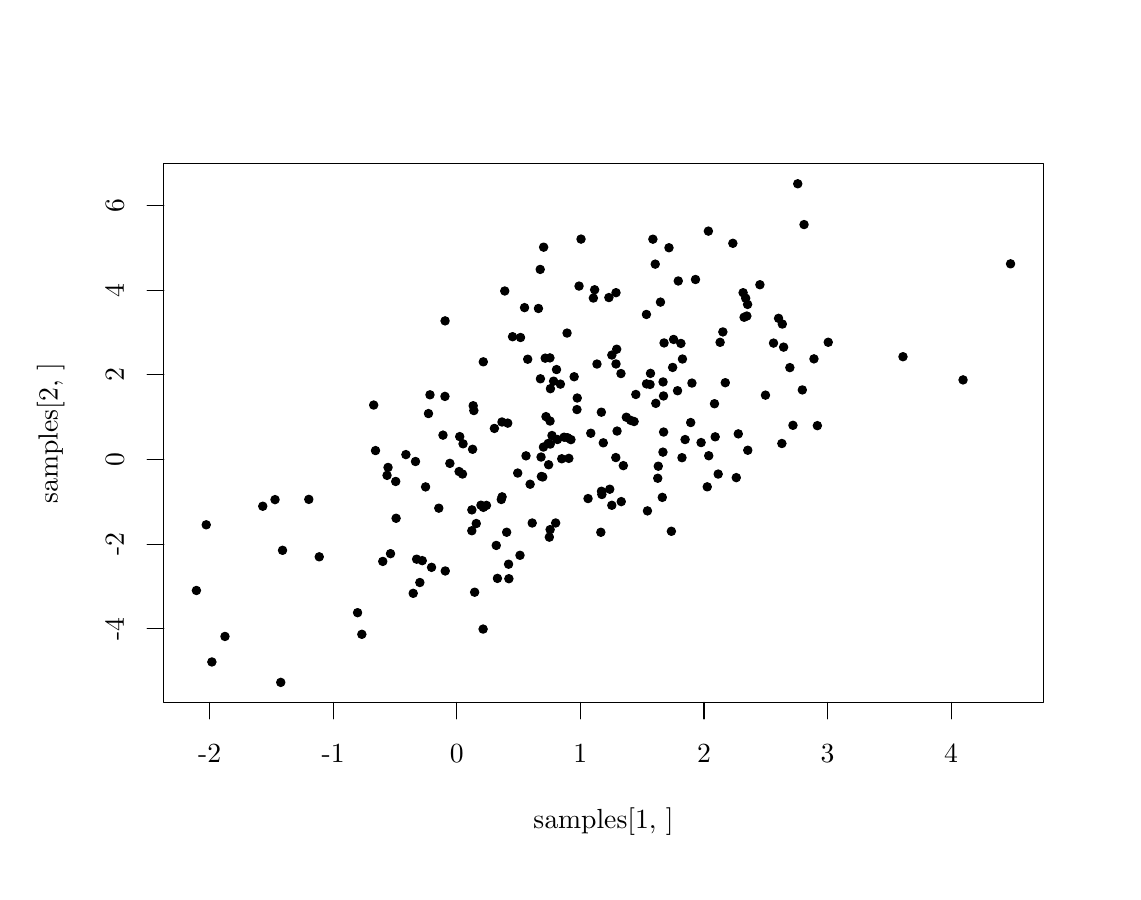
\begin{tikzpicture}[x=1pt,y=1pt]
\definecolor{fillColor}{RGB}{255,255,255}
\path[use as bounding box,fill=fillColor,fill opacity=0.00] (0,0) rectangle (392.13,304.99);
\begin{scope}
\path[clip] ( 49.20, 61.20) rectangle (366.93,255.79);
\definecolor{drawColor}{RGB}{0,0,0}
\definecolor{fillColor}{RGB}{0,0,0}

\path[draw=drawColor,line width= 0.4pt,line join=round,line cap=round,fill=fillColor] (191.10,181.44) circle (  1.50);

\path[draw=drawColor,line width= 0.4pt,line join=round,line cap=round,fill=fillColor] ( 92.09,116.13) circle (  1.50);

\path[draw=drawColor,line width= 0.4pt,line join=round,line cap=round,fill=fillColor] (225.92,228.56) circle (  1.50);

\path[draw=drawColor,line width= 0.4pt,line join=round,line cap=round,fill=fillColor] (207.30,166.04) circle (  1.50);

\path[draw=drawColor,line width= 0.4pt,line join=round,line cap=round,fill=fillColor] (177.07,144.05) circle (  1.50);

\path[draw=drawColor,line width= 0.4pt,line join=round,line cap=round,fill=fillColor] (185.51,149.83) circle (  1.50);

\path[draw=drawColor,line width= 0.4pt,line join=round,line cap=round,fill=fillColor] (188.83,154.52) circle (  1.50);

\path[draw=drawColor,line width= 0.4pt,line join=round,line cap=round,fill=fillColor] (181.56,140.01) circle (  1.50);

\path[draw=drawColor,line width= 0.4pt,line join=round,line cap=round,fill=fillColor] (226.97,169.24) circle (  1.50);

\path[draw=drawColor,line width= 0.4pt,line join=round,line cap=round,fill=fillColor] (180.68,185.18) circle (  1.50);

\path[draw=drawColor,line width= 0.4pt,line join=round,line cap=round,fill=fillColor] (271.33,199.96) circle (  1.50);

\path[draw=drawColor,line width= 0.4pt,line join=round,line cap=round,fill=fillColor] (228.66,205.82) circle (  1.50);

\path[draw=drawColor,line width= 0.4pt,line join=round,line cap=round,fill=fillColor] (215.24,146.73) circle (  1.50);

\path[draw=drawColor,line width= 0.4pt,line join=round,line cap=round,fill=fillColor] (130.22,146.08) circle (  1.50);

\path[draw=drawColor,line width= 0.4pt,line join=round,line cap=round,fill=fillColor] (205.71,183.44) circle (  1.50);

\path[draw=drawColor,line width= 0.4pt,line join=round,line cap=round,fill=fillColor] (279.92,174.09) circle (  1.50);

\path[draw=drawColor,line width= 0.4pt,line join=round,line cap=round,fill=fillColor] (141.71,104.50) circle (  1.50);

\path[draw=drawColor,line width= 0.4pt,line join=round,line cap=round,fill=fillColor] (212.98,159.22) circle (  1.50);

\path[draw=drawColor,line width= 0.4pt,line join=round,line cap=round,fill=fillColor] (236.04,190.89) circle (  1.50);

\path[draw=drawColor,line width= 0.4pt,line join=round,line cap=round,fill=fillColor] (232.60,123.01) circle (  1.50);

\path[draw=drawColor,line width= 0.4pt,line join=round,line cap=round,fill=fillColor] (208.00,154.97) circle (  1.50);

\path[draw=drawColor,line width= 0.4pt,line join=round,line cap=round,fill=fillColor] (125.03,168.62) circle (  1.50);

\path[draw=drawColor,line width= 0.4pt,line join=round,line cap=round,fill=fillColor] (229.55,151.61) circle (  1.50);

\path[draw=drawColor,line width= 0.4pt,line join=round,line cap=round,fill=fillColor] (179.54,203.83) circle (  1.50);

\path[draw=drawColor,line width= 0.4pt,line join=round,line cap=round,fill=fillColor] (101.59,134.54) circle (  1.50);

\path[draw=drawColor,line width= 0.4pt,line join=round,line cap=round,fill=fillColor] (236.60,185.25) circle (  1.50);

\path[draw=drawColor,line width= 0.4pt,line join=round,line cap=round,fill=fillColor] (243.34,155.06) circle (  1.50);

\path[draw=drawColor,line width= 0.4pt,line join=round,line cap=round,fill=fillColor] ( 66.56, 75.79) circle (  1.50);

\path[draw=drawColor,line width= 0.4pt,line join=round,line cap=round,fill=fillColor] (256.78,158.21) circle (  1.50);

\path[draw=drawColor,line width= 0.4pt,line join=round,line cap=round,fill=fillColor] (145.94,109.98) circle (  1.50);

\path[draw=drawColor,line width= 0.4pt,line join=round,line cap=round,fill=fillColor] (235.09,213.46) circle (  1.50);

\path[draw=drawColor,line width= 0.4pt,line join=round,line cap=round,fill=fillColor] (224.89,176.07) circle (  1.50);

\path[draw=drawColor,line width= 0.4pt,line join=round,line cap=round,fill=fillColor] (191.43,156.17) circle (  1.50);

\path[draw=drawColor,line width= 0.4pt,line join=round,line cap=round,fill=fillColor] (219.75,172.45) circle (  1.50);

\path[draw=drawColor,line width= 0.4pt,line join=round,line cap=round,fill=fillColor] (199.24,211.61) circle (  1.50);

\path[draw=drawColor,line width= 0.4pt,line join=round,line cap=round,fill=fillColor] (188.11,154.75) circle (  1.50);

\path[draw=drawColor,line width= 0.4pt,line join=round,line cap=round,fill=fillColor] (105.36,113.78) circle (  1.50);

\path[draw=drawColor,line width= 0.4pt,line join=round,line cap=round,fill=fillColor] (185.20,217.63) circle (  1.50);

\path[draw=drawColor,line width= 0.4pt,line join=round,line cap=round,fill=fillColor] (197.47,178.85) circle (  1.50);

\path[draw=drawColor,line width= 0.4pt,line join=round,line cap=round,fill=fillColor] (196.31,156.13) circle (  1.50);

\path[draw=drawColor,line width= 0.4pt,line join=round,line cap=round,fill=fillColor] (171.14,134.50) circle (  1.50);

\path[draw=drawColor,line width= 0.4pt,line join=round,line cap=round,fill=fillColor] (188.79,123.61) circle (  1.50);

\path[draw=drawColor,line width= 0.4pt,line join=round,line cap=round,fill=fillColor] (125.69,152.17) circle (  1.50);

\path[draw=drawColor,line width= 0.4pt,line join=round,line cap=round,fill=fillColor] (207.33,137.47) circle (  1.50);

\path[draw=drawColor,line width= 0.4pt,line join=round,line cap=round,fill=fillColor] (180.07,150.27) circle (  1.50);

\path[draw=drawColor,line width= 0.4pt,line join=round,line cap=round,fill=fillColor] (231.73,225.46) circle (  1.50);

\path[draw=drawColor,line width= 0.4pt,line join=round,line cap=round,fill=fillColor] (217.92,163.08) circle (  1.50);

\path[draw=drawColor,line width= 0.4pt,line join=round,line cap=round,fill=fillColor] (260.21,152.29) circle (  1.50);

\path[draw=drawColor,line width= 0.4pt,line join=round,line cap=round,fill=fillColor] (175.21,193.32) circle (  1.50);

\path[draw=drawColor,line width= 0.4pt,line join=round,line cap=round,fill=fillColor] (168.65,160.18) circle (  1.50);

\path[draw=drawColor,line width= 0.4pt,line join=round,line cap=round,fill=fillColor] (245.56,139.07) circle (  1.50);

\path[draw=drawColor,line width= 0.4pt,line join=round,line cap=round,fill=fillColor] (188.76,162.84) circle (  1.50);

\path[draw=drawColor,line width= 0.4pt,line join=round,line cap=round,fill=fillColor] (157.12,143.69) circle (  1.50);

\path[draw=drawColor,line width= 0.4pt,line join=round,line cap=round,fill=fillColor] (249.51,143.68) circle (  1.50);

\path[draw=drawColor,line width= 0.4pt,line join=round,line cap=round,fill=fillColor] (195.05,156.83) circle (  1.50);

\path[draw=drawColor,line width= 0.4pt,line join=round,line cap=round,fill=fillColor] (251.20,195.05) circle (  1.50);

\path[draw=drawColor,line width= 0.4pt,line join=round,line cap=round,fill=fillColor] (195.55,149.36) circle (  1.50);

\path[draw=drawColor,line width= 0.4pt,line join=round,line cap=round,fill=fillColor] (160.77,152.64) circle (  1.50);

\path[draw=drawColor,line width= 0.4pt,line join=round,line cap=round,fill=fillColor] ( 71.29, 85.01) circle (  1.50);

\path[draw=drawColor,line width= 0.4pt,line join=round,line cap=round,fill=fillColor] (142.58,112.40) circle (  1.50);

\path[draw=drawColor,line width= 0.4pt,line join=round,line cap=round,fill=fillColor] (184.56,203.52) circle (  1.50);

\path[draw=drawColor,line width= 0.4pt,line join=round,line cap=round,fill=fillColor] (178.09,193.03) circle (  1.50);

\path[draw=drawColor,line width= 0.4pt,line join=round,line cap=round,fill=fillColor] (150.07,157.75) circle (  1.50);

\path[draw=drawColor,line width= 0.4pt,line join=round,line cap=round,fill=fillColor] (233.06,182.22) circle (  1.50);

\path[draw=drawColor,line width= 0.4pt,line join=round,line cap=round,fill=fillColor] (203.48,158.44) circle (  1.50);

\path[draw=drawColor,line width= 0.4pt,line join=round,line cap=round,fill=fillColor] (260.14,204.98) circle (  1.50);

\path[draw=drawColor,line width= 0.4pt,line join=round,line cap=round,fill=fillColor] (129.86,143.22) circle (  1.50);

\path[draw=drawColor,line width= 0.4pt,line join=round,line cap=round,fill=fillColor] (187.01,185.57) circle (  1.50);

\path[draw=drawColor,line width= 0.4pt,line join=round,line cap=round,fill=fillColor] (173.77,111.11) circle (  1.50);

\path[draw=drawColor,line width= 0.4pt,line join=round,line cap=round,fill=fillColor] (188.89,174.54) circle (  1.50);

\path[draw=drawColor,line width= 0.4pt,line join=round,line cap=round,fill=fillColor] ( 91.45, 68.41) circle (  1.50);

\path[draw=drawColor,line width= 0.4pt,line join=round,line cap=round,fill=fillColor] (160.49,123.21) circle (  1.50);

\path[draw=drawColor,line width= 0.4pt,line join=round,line cap=round,fill=fillColor] (252.08,176.70) circle (  1.50);

\path[draw=drawColor,line width= 0.4pt,line join=round,line cap=round,fill=fillColor] (164.57, 87.67) circle (  1.50);

\path[draw=drawColor,line width= 0.4pt,line join=round,line cap=round,fill=fillColor] (152.56,147.55) circle (  1.50);

\path[draw=drawColor,line width= 0.4pt,line join=round,line cap=round,fill=fillColor] (338.00,177.71) circle (  1.50);

\path[draw=drawColor,line width= 0.4pt,line join=round,line cap=round,fill=fillColor] (165.78,132.36) circle (  1.50);

\path[draw=drawColor,line width= 0.4pt,line join=round,line cap=round,fill=fillColor] (140.14,148.22) circle (  1.50);

\path[draw=drawColor,line width= 0.4pt,line join=round,line cap=round,fill=fillColor] (173.08,122.66) circle (  1.50);

\path[draw=drawColor,line width= 0.4pt,line join=round,line cap=round,fill=fillColor] (187.29,164.44) circle (  1.50);

\path[draw=drawColor,line width= 0.4pt,line join=round,line cap=round,fill=fillColor] (248.43,157.14) circle (  1.50);

\path[draw=drawColor,line width= 0.4pt,line join=round,line cap=round,fill=fillColor] (227.67,142.17) circle (  1.50);

\path[draw=drawColor,line width= 0.4pt,line join=round,line cap=round,fill=fillColor] (190.04,177.25) circle (  1.50);

\path[draw=drawColor,line width= 0.4pt,line join=round,line cap=round,fill=fillColor] (199.95,228.59) circle (  1.50);

\path[draw=drawColor,line width= 0.4pt,line join=round,line cap=round,fill=fillColor] (188.24,147.05) circle (  1.50);

\path[draw=drawColor,line width= 0.4pt,line join=round,line cap=round,fill=fillColor] ( 84.95,132.06) circle (  1.50);

\path[draw=drawColor,line width= 0.4pt,line join=round,line cap=round,fill=fillColor] (185.28,178.11) circle (  1.50);

\path[draw=drawColor,line width= 0.4pt,line join=round,line cap=round,fill=fillColor] (227.87,146.53) circle (  1.50);

\path[draw=drawColor,line width= 0.4pt,line join=round,line cap=round,fill=fillColor] (273.15,189.55) circle (  1.50);

\path[draw=drawColor,line width= 0.4pt,line join=round,line cap=round,fill=fillColor] (190.78,126.01) circle (  1.50);

\path[draw=drawColor,line width= 0.4pt,line join=round,line cap=round,fill=fillColor] (161.22,166.63) circle (  1.50);

\path[draw=drawColor,line width= 0.4pt,line join=round,line cap=round,fill=fillColor] ( 60.97,101.62) circle (  1.50);

\path[draw=drawColor,line width= 0.4pt,line join=round,line cap=round,fill=fillColor] (210.02,207.46) circle (  1.50);

\path[draw=drawColor,line width= 0.4pt,line join=round,line cap=round,fill=fillColor] (223.61,176.28) circle (  1.50);

\path[draw=drawColor,line width= 0.4pt,line join=round,line cap=round,fill=fillColor] (207.48,136.30) circle (  1.50);

\path[draw=drawColor,line width= 0.4pt,line join=round,line cap=round,fill=fillColor] (160.98,168.38) circle (  1.50);

\path[draw=drawColor,line width= 0.4pt,line join=round,line cap=round,fill=fillColor] (229.76,171.91) circle (  1.50);

\path[draw=drawColor,line width= 0.4pt,line join=round,line cap=round,fill=fillColor] (225.05,180.07) circle (  1.50);

\path[draw=drawColor,line width= 0.4pt,line join=round,line cap=round,fill=fillColor] (236.43,149.60) circle (  1.50);

\path[draw=drawColor,line width= 0.4pt,line join=round,line cap=round,fill=fillColor] (193.83,157.01) circle (  1.50);

\path[draw=drawColor,line width= 0.4pt,line join=round,line cap=round,fill=fillColor] (145.37,172.32) circle (  1.50);

\path[draw=drawColor,line width= 0.4pt,line join=round,line cap=round,fill=fillColor] ( 89.38,134.45) circle (  1.50);

\path[draw=drawColor,line width= 0.4pt,line join=round,line cap=round,fill=fillColor] (207.11,122.65) circle (  1.50);

\path[draw=drawColor,line width= 0.4pt,line join=round,line cap=round,fill=fillColor] (132.99,141.01) circle (  1.50);

\path[draw=drawColor,line width= 0.4pt,line join=round,line cap=round,fill=fillColor] (256.05,142.40) circle (  1.50);

\path[draw=drawColor,line width= 0.4pt,line join=round,line cap=round,fill=fillColor] (214.49,133.73) circle (  1.50);

\path[draw=drawColor,line width= 0.4pt,line join=round,line cap=round,fill=fillColor] (185.63,142.82) circle (  1.50);

\path[draw=drawColor,line width= 0.4pt,line join=round,line cap=round,fill=fillColor] (211.08,132.40) circle (  1.50);

\path[draw=drawColor,line width= 0.4pt,line join=round,line cap=round,fill=fillColor] (278.26,248.58) circle (  1.50);

\path[draw=drawColor,line width= 0.4pt,line join=round,line cap=round,fill=fillColor] (172.39,209.84) circle (  1.50);

\path[draw=drawColor,line width= 0.4pt,line join=round,line cap=round,fill=fillColor] (162.10,125.81) circle (  1.50);

\path[draw=drawColor,line width= 0.4pt,line join=round,line cap=round,fill=fillColor] (212.84,188.80) circle (  1.50);

\path[draw=drawColor,line width= 0.4pt,line join=round,line cap=round,fill=fillColor] (229.79,158.87) circle (  1.50);

\path[draw=drawColor,line width= 0.4pt,line join=round,line cap=round,fill=fillColor] (140.55,112.93) circle (  1.50);

\path[draw=drawColor,line width= 0.4pt,line join=round,line cap=round,fill=fillColor] (254.81,227.07) circle (  1.50);

\path[draw=drawColor,line width= 0.4pt,line join=round,line cap=round,fill=fillColor] (275.41,182.15) circle (  1.50);

\path[draw=drawColor,line width= 0.4pt,line join=round,line cap=round,fill=fillColor] (188.71,185.66) circle (  1.50);

\path[draw=drawColor,line width= 0.4pt,line join=round,line cap=round,fill=fillColor] (136.67,150.72) circle (  1.50);

\path[draw=drawColor,line width= 0.4pt,line join=round,line cap=round,fill=fillColor] (219.13,162.67) circle (  1.50);

\path[draw=drawColor,line width= 0.4pt,line join=round,line cap=round,fill=fillColor] (173.47,162.09) circle (  1.50);

\path[draw=drawColor,line width= 0.4pt,line join=round,line cap=round,fill=fillColor] (171.43,135.45) circle (  1.50);

\path[draw=drawColor,line width= 0.4pt,line join=round,line cap=round,fill=fillColor] (241.32,213.99) circle (  1.50);

\path[draw=drawColor,line width= 0.4pt,line join=round,line cap=round,fill=fillColor] (186.44,225.67) circle (  1.50);

\path[draw=drawColor,line width= 0.4pt,line join=round,line cap=round,fill=fillColor] (202.49,134.83) circle (  1.50);

\path[draw=drawColor,line width= 0.4pt,line join=round,line cap=round,fill=fillColor] (246.10,150.31) circle (  1.50);

\path[draw=drawColor,line width= 0.4pt,line join=round,line cap=round,fill=fillColor] (212.52,149.65) circle (  1.50);

\path[draw=drawColor,line width= 0.4pt,line join=round,line cap=round,fill=fillColor] (161.51,100.99) circle (  1.50);

\path[draw=drawColor,line width= 0.4pt,line join=round,line cap=round,fill=fillColor] (148.56,131.36) circle (  1.50);

\path[draw=drawColor,line width= 0.4pt,line join=round,line cap=round,fill=fillColor] (189.45,157.61) circle (  1.50);

\path[draw=drawColor,line width= 0.4pt,line join=round,line cap=round,fill=fillColor] (226.77,219.54) circle (  1.50);

\path[draw=drawColor,line width= 0.4pt,line join=round,line cap=round,fill=fillColor] (164.65,131.66) circle (  1.50);

\path[draw=drawColor,line width= 0.4pt,line join=round,line cap=round,fill=fillColor] (259.87,200.79) circle (  1.50);

\path[draw=drawColor,line width= 0.4pt,line join=round,line cap=round,fill=fillColor] (269.51,191.01) circle (  1.50);

\path[draw=drawColor,line width= 0.4pt,line join=round,line cap=round,fill=fillColor] (128.31,112.12) circle (  1.50);

\path[draw=drawColor,line width= 0.4pt,line join=round,line cap=round,fill=fillColor] (156.12,157.22) circle (  1.50);

\path[draw=drawColor,line width= 0.4pt,line join=round,line cap=round,fill=fillColor] (276.53,161.30) circle (  1.50);

\path[draw=drawColor,line width= 0.4pt,line join=round,line cap=round,fill=fillColor] (316.29,186.09) circle (  1.50);

\path[draw=drawColor,line width= 0.4pt,line join=round,line cap=round,fill=fillColor] (223.95,130.38) circle (  1.50);

\path[draw=drawColor,line width= 0.4pt,line join=round,line cap=round,fill=fillColor] (186.36,153.44) circle (  1.50);

\path[draw=drawColor,line width= 0.4pt,line join=round,line cap=round,fill=fillColor] (237.56,156.15) circle (  1.50);

\path[draw=drawColor,line width= 0.4pt,line join=round,line cap=round,fill=fillColor] (155.90,144.59) circle (  1.50);

\path[draw=drawColor,line width= 0.4pt,line join=round,line cap=round,fill=fillColor] (258.52,209.22) circle (  1.50);

\path[draw=drawColor,line width= 0.4pt,line join=round,line cap=round,fill=fillColor] (223.58,201.36) circle (  1.50);

\path[draw=drawColor,line width= 0.4pt,line join=round,line cap=round,fill=fillColor] (212.59,209.23) circle (  1.50);

\path[draw=drawColor,line width= 0.4pt,line join=round,line cap=round,fill=fillColor] (272.52,154.73) circle (  1.50);

\path[draw=drawColor,line width= 0.4pt,line join=round,line cap=round,fill=fillColor] (216.33,164.22) circle (  1.50);

\path[draw=drawColor,line width= 0.4pt,line join=round,line cap=round,fill=fillColor] (120.75, 85.78) circle (  1.50);

\path[draw=drawColor,line width= 0.4pt,line join=round,line cap=round,fill=fillColor] (150.89,108.67) circle (  1.50);

\path[draw=drawColor,line width= 0.4pt,line join=round,line cap=round,fill=fillColor] (160.51,130.74) circle (  1.50);

\path[draw=drawColor,line width= 0.4pt,line join=round,line cap=round,fill=fillColor] (240.02,176.56) circle (  1.50);

\path[draw=drawColor,line width= 0.4pt,line join=round,line cap=round,fill=fillColor] (204.87,210.28) circle (  1.50);

\path[draw=drawColor,line width= 0.4pt,line join=round,line cap=round,fill=fillColor] (192.98,149.21) circle (  1.50);

\path[draw=drawColor,line width= 0.4pt,line join=round,line cap=round,fill=fillColor] (250.21,191.29) circle (  1.50);

\path[draw=drawColor,line width= 0.4pt,line join=round,line cap=round,fill=fillColor] (210.33,138.21) circle (  1.50);

\path[draw=drawColor,line width= 0.4pt,line join=round,line cap=round,fill=fillColor] (289.28,191.31) circle (  1.50);

\path[draw=drawColor,line width= 0.4pt,line join=round,line cap=round,fill=fillColor] (131.11,114.92) circle (  1.50);

\path[draw=drawColor,line width= 0.4pt,line join=round,line cap=round,fill=fillColor] (258.88,200.35) circle (  1.50);

\path[draw=drawColor,line width= 0.4pt,line join=round,line cap=round,fill=fillColor] (272.69,197.88) circle (  1.50);

\path[draw=drawColor,line width= 0.4pt,line join=round,line cap=round,fill=fillColor] (150.78,171.75) circle (  1.50);

\path[draw=drawColor,line width= 0.4pt,line join=round,line cap=round,fill=fillColor] (280.54,233.84) circle (  1.50);

\path[draw=drawColor,line width= 0.4pt,line join=round,line cap=round,fill=fillColor] (177.90,114.33) circle (  1.50);

\path[draw=drawColor,line width= 0.4pt,line join=round,line cap=round,fill=fillColor] (234.83,173.80) circle (  1.50);

\path[draw=drawColor,line width= 0.4pt,line join=round,line cap=round,fill=fillColor] (259.45,207.23) circle (  1.50);

\path[draw=drawColor,line width= 0.4pt,line join=round,line cap=round,fill=fillColor] (285.35,161.18) circle (  1.50);

\path[draw=drawColor,line width= 0.4pt,line join=round,line cap=round,fill=fillColor] (229.32,135.26) circle (  1.50);

\path[draw=drawColor,line width= 0.4pt,line join=round,line cap=round,fill=fillColor] (139.31,100.59) circle (  1.50);

\path[draw=drawColor,line width= 0.4pt,line join=round,line cap=round,fill=fillColor] (229.96,191.07) circle (  1.50);

\path[draw=drawColor,line width= 0.4pt,line join=round,line cap=round,fill=fillColor] (157.33,154.61) circle (  1.50);

\path[draw=drawColor,line width= 0.4pt,line join=round,line cap=round,fill=fillColor] (239.58,162.30) circle (  1.50);

\path[draw=drawColor,line width= 0.4pt,line join=round,line cap=round,fill=fillColor] (169.32,117.90) circle (  1.50);

\path[draw=drawColor,line width= 0.4pt,line join=round,line cap=round,fill=fillColor] (186.12,142.64) circle (  1.50);

\path[draw=drawColor,line width= 0.4pt,line join=round,line cap=round,fill=fillColor] (144.83,165.54) circle (  1.50);

\path[draw=drawColor,line width= 0.4pt,line join=round,line cap=round,fill=fillColor] (245.97,231.47) circle (  1.50);

\path[draw=drawColor,line width= 0.4pt,line join=round,line cap=round,fill=fillColor] (233.40,192.33) circle (  1.50);

\path[draw=drawColor,line width= 0.4pt,line join=round,line cap=round,fill=fillColor] (198.48,166.99) circle (  1.50);

\path[draw=drawColor,line width= 0.4pt,line join=round,line cap=round,fill=fillColor] (194.91,194.63) circle (  1.50);

\path[draw=drawColor,line width= 0.4pt,line join=round,line cap=round,fill=fillColor] (192.49,176.18) circle (  1.50);

\path[draw=drawColor,line width= 0.4pt,line join=round,line cap=round,fill=fillColor] (212.59,183.47) circle (  1.50);

\path[draw=drawColor,line width= 0.4pt,line join=round,line cap=round,fill=fillColor] (163.79,132.44) circle (  1.50);

\path[draw=drawColor,line width= 0.4pt,line join=round,line cap=round,fill=fillColor] (204.41,207.28) circle (  1.50);

\path[draw=drawColor,line width= 0.4pt,line join=round,line cap=round,fill=fillColor] (229.60,176.98) circle (  1.50);

\path[draw=drawColor,line width= 0.4pt,line join=round,line cap=round,fill=fillColor] (214.38,180.00) circle (  1.50);

\path[draw=drawColor,line width= 0.4pt,line join=round,line cap=round,fill=fillColor] (119.21, 93.60) circle (  1.50);

\path[draw=drawColor,line width= 0.4pt,line join=round,line cap=round,fill=fillColor] (143.78,139.05) circle (  1.50);

\path[draw=drawColor,line width= 0.4pt,line join=round,line cap=round,fill=fillColor] (248.18,169.10) circle (  1.50);

\path[draw=drawColor,line width= 0.4pt,line join=round,line cap=round,fill=fillColor] (284.12,185.31) circle (  1.50);

\path[draw=drawColor,line width= 0.4pt,line join=round,line cap=round,fill=fillColor] (355.16,219.65) circle (  1.50);

\path[draw=drawColor,line width= 0.4pt,line join=round,line cap=round,fill=fillColor] (188.50,120.89) circle (  1.50);

\path[draw=drawColor,line width= 0.4pt,line join=round,line cap=round,fill=fillColor] (171.38,162.50) circle (  1.50);

\path[draw=drawColor,line width= 0.4pt,line join=round,line cap=round,fill=fillColor] (133.13,127.71) circle (  1.50);

\path[draw=drawColor,line width= 0.4pt,line join=round,line cap=round,fill=fillColor] (266.60,172.20) circle (  1.50);

\path[draw=drawColor,line width= 0.4pt,line join=round,line cap=round,fill=fillColor] (164.64,184.24) circle (  1.50);

\path[draw=drawColor,line width= 0.4pt,line join=round,line cap=round,fill=fillColor] (150.83,199.04) circle (  1.50);

\path[draw=drawColor,line width= 0.4pt,line join=round,line cap=round,fill=fillColor] (211.09,186.69) circle (  1.50);

\path[draw=drawColor,line width= 0.4pt,line join=round,line cap=round,fill=fillColor] (182.31,126.00) circle (  1.50);

\path[draw=drawColor,line width= 0.4pt,line join=round,line cap=round,fill=fillColor] (264.59,212.10) circle (  1.50);

\path[draw=drawColor,line width= 0.4pt,line join=round,line cap=round,fill=fillColor] (173.88,105.87) circle (  1.50);

\path[draw=drawColor,line width= 0.4pt,line join=round,line cap=round,fill=fillColor] (198.58,171.17) circle (  1.50);

\path[draw=drawColor,line width= 0.4pt,line join=round,line cap=round,fill=fillColor] (169.74,105.99) circle (  1.50);

\path[draw=drawColor,line width= 0.4pt,line join=round,line cap=round,fill=fillColor] ( 64.52,125.35) circle (  1.50);
\end{scope}
\begin{scope}
\path[clip] (  0.00,  0.00) rectangle (392.13,304.99);
\definecolor{drawColor}{RGB}{0,0,0}

\path[draw=drawColor,line width= 0.4pt,line join=round,line cap=round] ( 65.76, 61.20) -- (333.68, 61.20);

\path[draw=drawColor,line width= 0.4pt,line join=round,line cap=round] ( 65.76, 61.20) -- ( 65.76, 55.20);

\path[draw=drawColor,line width= 0.4pt,line join=round,line cap=round] (110.41, 61.20) -- (110.41, 55.20);

\path[draw=drawColor,line width= 0.4pt,line join=round,line cap=round] (155.07, 61.20) -- (155.07, 55.20);

\path[draw=drawColor,line width= 0.4pt,line join=round,line cap=round] (199.72, 61.20) -- (199.72, 55.20);

\path[draw=drawColor,line width= 0.4pt,line join=round,line cap=round] (244.37, 61.20) -- (244.37, 55.20);

\path[draw=drawColor,line width= 0.4pt,line join=round,line cap=round] (289.03, 61.20) -- (289.03, 55.20);

\path[draw=drawColor,line width= 0.4pt,line join=round,line cap=round] (333.68, 61.20) -- (333.68, 55.20);

\node[text=drawColor,anchor=base,inner sep=0pt, outer sep=0pt, scale=  1.00] at ( 65.76, 39.60) {-2};

\node[text=drawColor,anchor=base,inner sep=0pt, outer sep=0pt, scale=  1.00] at (110.41, 39.60) {-1};

\node[text=drawColor,anchor=base,inner sep=0pt, outer sep=0pt, scale=  1.00] at (155.07, 39.60) {0};

\node[text=drawColor,anchor=base,inner sep=0pt, outer sep=0pt, scale=  1.00] at (199.72, 39.60) {1};

\node[text=drawColor,anchor=base,inner sep=0pt, outer sep=0pt, scale=  1.00] at (244.37, 39.60) {2};

\node[text=drawColor,anchor=base,inner sep=0pt, outer sep=0pt, scale=  1.00] at (289.03, 39.60) {3};

\node[text=drawColor,anchor=base,inner sep=0pt, outer sep=0pt, scale=  1.00] at (333.68, 39.60) {4};

\path[draw=drawColor,line width= 0.4pt,line join=round,line cap=round] ( 49.20, 87.77) -- ( 49.20,240.70);

\path[draw=drawColor,line width= 0.4pt,line join=round,line cap=round] ( 49.20, 87.77) -- ( 43.20, 87.77);

\path[draw=drawColor,line width= 0.4pt,line join=round,line cap=round] ( 49.20,118.36) -- ( 43.20,118.36);

\path[draw=drawColor,line width= 0.4pt,line join=round,line cap=round] ( 49.20,148.95) -- ( 43.20,148.95);

\path[draw=drawColor,line width= 0.4pt,line join=round,line cap=round] ( 49.20,179.53) -- ( 43.20,179.53);

\path[draw=drawColor,line width= 0.4pt,line join=round,line cap=round] ( 49.20,210.12) -- ( 43.20,210.12);

\path[draw=drawColor,line width= 0.4pt,line join=round,line cap=round] ( 49.20,240.70) -- ( 43.20,240.70);

\node[text=drawColor,rotate= 90.00,anchor=base,inner sep=0pt, outer sep=0pt, scale=  1.00] at ( 34.80, 87.77) {-4};

\node[text=drawColor,rotate= 90.00,anchor=base,inner sep=0pt, outer sep=0pt, scale=  1.00] at ( 34.80,118.36) {-2};

\node[text=drawColor,rotate= 90.00,anchor=base,inner sep=0pt, outer sep=0pt, scale=  1.00] at ( 34.80,148.95) {0};

\node[text=drawColor,rotate= 90.00,anchor=base,inner sep=0pt, outer sep=0pt, scale=  1.00] at ( 34.80,179.53) {2};

\node[text=drawColor,rotate= 90.00,anchor=base,inner sep=0pt, outer sep=0pt, scale=  1.00] at ( 34.80,210.12) {4};

\node[text=drawColor,rotate= 90.00,anchor=base,inner sep=0pt, outer sep=0pt, scale=  1.00] at ( 34.80,240.70) {6};

\path[draw=drawColor,line width= 0.4pt,line join=round,line cap=round] ( 49.20, 61.20) --
	(366.93, 61.20) --
	(366.93,255.79) --
	( 49.20,255.79) --
	( 49.20, 61.20);
\end{scope}
\begin{scope}
\path[clip] (  0.00,  0.00) rectangle (392.13,304.99);
\definecolor{drawColor}{RGB}{0,0,0}

\node[text=drawColor,anchor=base,inner sep=0pt, outer sep=0pt, scale=  1.00] at (208.06, 15.60) {samples[1, ]};

\node[text=drawColor,rotate= 90.00,anchor=base,inner sep=0pt, outer sep=0pt, scale=  1.00] at ( 10.80,158.49) {samples[2, ]};
\end{scope}
\end{tikzpicture}

	\caption{Projection on the $xy$-plane of the sample from the multivariate normal distribution}
	\label{fig:sample}
\end{figure}

\section*{Acknowledgements}
Rune Buckinx and Michaël Maex for helping to fix stupid mistakes in stupid R code
Seppe for stupid discussions about how well the questions are asked
Thibeau for organising a group crying session
Robbe for genuinly good input about trying to solve stupid questions


%\printinunitsof{in}\prntlen{\textwidth}


\end{document}
